\documentclass{article}

% if you need to pass options to natbib, use, e.g.:
%     \PassOptionsToPackage{numbers, compress}{natbib}
% before loading neurips_2020

% ready for submission
% \usepackage{neurips_2020}

% to compile a preprint version, e.g., for submission to arXiv, add add the
% [preprint] option:
%     \usepackage[preprint]{neurips_2020}

% to compile a camera-ready version, add the [final] option, e.g.:
%     \usepackage[final]{neurips_2020}

% to avoid loading the natbib package, add option nonatbib:
\usepackage{neurips_2020}

\usepackage[utf8]{inputenc} % allow utf-8 input
\usepackage[T1]{fontenc}    % use 8-bit T1 fonts
\usepackage{hyperref}       % hyperlinks
\usepackage{url}            % simple URL typesetting
\usepackage{booktabs}       % professional-quality tables
\usepackage{amsfonts}       % blackboard math symbols
\usepackage{nicefrac}       % compact symbols for 1/2, etc.
\usepackage{microtype}      % microtypography
\usepackage{amsmath, amsfonts, amssymb, amsthm}

\usepackage{color}
\definecolor{darkblue}{rgb}{0.0,0.0,0.2}
\hypersetup{colorlinks,breaklinks,
	linkcolor=darkblue,urlcolor=darkblue,
	anchorcolor=darkblue,citecolor=darkblue}
\usepackage{wrapfig}
\usepackage{subcaption}
\usepackage[colorinlistoftodos,textsize=tiny]{todonotes} % need xargs for below
%\usepackage{accents}
\usepackage{bbm}
\usepackage{xspace}

\newcommand{\Comments}{1}
\newcommand{\mynote}[2]{\ifnum\Comments=1\textcolor{#1}{#2}\fi}
\newcommand{\mytodo}[2]{\ifnum\Comments=1%
	\todo[linecolor=#1!80!black,backgroundcolor=#1,bordercolor=#1!80!black]{#2}\fi}
\newcommand{\raf}[1]{\mynote{green!80!blue}{[RF: #1]}}
\newcommand{\raft}[1]{\mytodo{green!20!white}{RF: #1}}
\newcommand{\jessie}[1]{\mynote{purple}{[JF: #1]}}
\newcommand{\jessiet}[1]{\mytodo{purple!20!white}{JF: #1}}
\newcommand{\proposedadd}[1]{\mynote{orange}{#1}}
\newcommand{\bo}[1]{\mynote{blue}{[Bo: #1]}}
\newcommand{\botodo}[1]{\mytodo{blue!20!white}{[Bo: #1]}}
\newcommand{\btw}[1]{\mytodo{gray!20!white}{[BTW: #1]}}%TURN OFF FOR NOW \mytodo{gray}{#1}}
\ifnum\Comments=1               % fix margins for todonotes
\setlength{\marginparwidth}{1in}
\fi

\newcommand{\reals}{\mathbb{R}}
\newcommand{\posreals}{\reals_{>0}}%{\reals_{++}}
\newcommand{\simplex}{\Delta_\Y}
\newcommand{\relint}[1]{\mathrm{relint}(#1)}
\newcommand{\prop}[1]{\mathrm{prop}[#1]}
\newcommand{\elic}{\mathrm{elic}}
\newcommand{\eliccvx}{\mathrm{elic}_\mathrm{cvx}}
\newcommand{\elicpoly}{\mathrm{elic}_\mathrm{pcvx}}
\newcommand{\elicembed}{\mathrm{elic}_\mathrm{embed}}
\newcommand{\ccdim}{\mathrm{cc\,dim}}
\newcommand{\codim}{\mathrm{codim}}
\newcommand{\rank}{\mathrm{rank}}
\newcommand{\supp}{\mathrm{supp}}
\newcommand{\spn}{\mathrm{span}}
\newcommand{\propdis}{\mu}
\newcommand{\affhull}{\mathrm{affhull}}


\newcommand{\C}{\mathcal{C}}
\newcommand{\D}{\mathcal{D}}
\newcommand{\E}{\mathbb{E}}
\newcommand{\F}{\mathcal{F}}
\newcommand{\I}{\mathcal{I}}
\newcommand{\N}{\mathcal{N}}
\newcommand{\R}{\mathcal{R}}
\renewcommand{\P}{\mathcal{P}}
\newcommand{\Sc}{\mathcal{S}}  % jessie, feel free to redef, just not \S :-)
\newcommand{\U}{\mathcal{U}}
\newcommand{\X}{\mathcal{X}}
\newcommand{\Y}{\mathcal{Y}}


\newcommand{\risk}[1]{#1^*}
\newcommand{\inprod}[2]{\langle #1, #2 \rangle}
\newcommand{\toto}{\rightrightarrows}
\newcommand{\ones}{\mathbbm{1}}

\newtheorem{theorem}{Theorem}
\newtheorem{lemma}{Lemma}
\newtheorem{proposition}{Proposition}
\newtheorem{corollary}{Corollary}
\newtheorem{conjecture}{Conjecture}
\newtheorem{definition}{Definition}
\newtheorem{assumption}{Assumption}
\newtheorem{remark}{Remark}


\DeclareMathOperator*{\argmax}{arg\,max}
\DeclareMathOperator*{\argmin}{arg\,min}
\DeclareMathOperator*{\arginf}{arg\,inf}
\DeclareMathOperator*{\sgn}{sgn}

\title{Indirect elicitation as a necessary condition for consistent surrogate losses}

% The \author macro works with any number of authors. There are two commands
% used to separate the names and addresses of multiple authors: \And and \AND.
%
% Using \And between authors leaves it to LaTeX to determine where to break the
% lines. Using \AND forces a line break at that point. So, if LaTeX puts 3 of 4
% authors names on the first line, and the last on the second line, try using
% \AND instead of \And before the third author name.

\author{%
  Jessie Finocchiaro\\
%  Department of Computer Science\\
  CU Boulder\\
  \texttt{jefi8453@colorado.edu} 
  % examples of more authors
  \And
   Rafael Frongillo\\
%   Department of Computer Science\\
   CU Boulder\\
  % Address \\
   \texttt{raf@colorado.edu} 
   \And
   Bo Waggoner\\
%   Department of Computer Science\\
   CU Boulder \\
  % Address \\
   \texttt{bwag@colorado.edu} 
  % \And
  % Coauthor \\
  % Affiliation \\
  % Address \\
  % \texttt{email} \\
  % \And
  % Coauthor \\
  % Affiliation \\
  % Address \\
  % \texttt{email} \\
}



\begin{document}

\maketitle

\begin{abstract}
Given a prediction task, understanding when one can and cannot design a consistent convex surrogate loss, particularly a low-dimensional one, is an important and active area of machine learning research. 
While calibration has historically been used to reason about consistency, we propose indirect property elicitation as an alternative necessary condition for a surrogate loss to be consistent. 
Motivated by structured prediction and other domains where the prediction dimension of the surrogate is of central importance, we give a novel lower bound on the prediction dimension. 
Our lower bound tightens existing results in the case of discrete predictions, namely the feasible subspace dimension, showing that previous work implicitly relied on calibration only via property elicitation. 
For continuous predictions, our lower bound gives new results for variance estimation as well as the estimation of entropy and norms of the conditional distribution.
\end{abstract}

\section{Introduction}\label{sec:intro}
\raf{General comment: see if you can make the intro less of an explanation to someone who has never heard of consistency, etc, and more of a ``reminder'' and recap of what's been going on in the field, culminating in the gap between what is out there and what we would like to know -- the gap that we fill}
\raf{General style: see if you can make the writing sharper, with less passive voice.  See if you can channel some Hemmingway and boil each sentence down to the key point.}
\jessie{Alright, I tried...}
In supervised machine learning, one often makes predictions about future outcomes by minimizing a surrogate loss on training data.
\bo{Reworded slightly.}
The use of a surrogate is often necessary for one of two reasons: the target loss does not satisfy some ``niceness'' conditions that we desire, or the goal is to estimate some statistic rather than minimize some target loss.
When given a target loss, a surrogate should yield good statistical guarantees; informally, we want low surrogate risk to imply low target risk.
%A good surrogate should yield bounds on the excess risk so that optimal predictions for the surrogate can be linked to optimal predictions for a target (possibly discrete) loss with bounded excess error, regardless of the underlying data distribution.
%\raft{Style example: ``we want low surrogate risk to mean low target risk.''}
In continuous estimation settings, one typically starts with a statistic of the data they would like to estimate instead of a target loss, such as the conditional expected value or an $\alpha$-quantile.
Here, we generalize consistency to make sense in target loss-less contexts (Definition~\ref{def:consistent-prop}).
%For example, if one wants to estimate the $\alpha$-quantile, they can do so by minimizing pinball loss over their data, but it is often unclear \emph{why} pinball loss is good for this prediction task.
\raft{I think few ML people know anything about pinball loss... I think we should de-emphasize the continuous setting in the intro, and include it in passing.}\jessiet{Removed the sentence, but probably want to at least allude to it?}
We desire a surrogate to be \emph{consistent}: a precursor to excess risk bounds and rates.
\raft{we desire \emph{consistency}, a precursor to excess risk bounds and rates}\jessiet{Changed}
We are particularly interested in consistent \emph{and convex} surrogates% in which any sequence of hypotheses converging to the optimal prediction can be linked to a sequence that converges to either the correct prediction for the discrete loss or statistic value, depending on the setting. 
%We would also like our surrogate losses to be 
that are efficient in the dimension of the prediction, as this is one potential source of significant computational speedup.

%\raf{Maybe start with ``in this paper, we'' or similar, and recap the high-level contributions.  E.g. ``Our results give two contributions to this field.  First, .....  Second, .....''  Something like that before going into the theorems.}

\bo{Reworded to avoid saying our findings are major -- some people won't like that.}\jessie{Good point}
Our results make two contributions to this field.
First, we show that indirect property elicitation is a necessary condition for consistency (Theorem~\ref{thm:consistent-implies-indir-elic}).
This lets us use property elicitation to bound the minimum prediction dimension needed to construct a consistent convex surrogate.
Previous lower bounds on the dimension of a consistent convex surrogate for a given task have been considered in one of four settings: whether one is given a target loss or not, and whether one is making a continuous or discrete prediction.
The bounds we show in our second contribution (Theorem~\ref{thm:cvx-flats}) are general enough to apply across all four settings, and is the first bound to our knowledge to handle this generality.


%We typically use convex surrogate loss functions that take some input $u \in \reals^d$ and measure error against the observed outcome $y \in \Y$.
%The value $d$ provides some notion of efficiency for the surrogate, as low-dimensional convex losses can improve the efficiency of the optimization algorithm.
%\cite{frongillo2015elicitation} pose an open question regarding a general characterization of the efficiency of \emph{convex elicitable properties}, which we show is bounded by finding the minimum dimension $d$ for which a consistent, convex loss can be constructed for the task at hand.

\raf{I'm usually against these sorts of sections if they are truly just a roadmap.  See if you can make it flow less like a table of contents and more like a list of contributions with references to where in the paper to find them.  E.g.\ ``After reviewing previous work and introducing our notation (\S X) we lay down a new general definition of consistency which can simultaneously capture all four settings above (\S Y).''} \jessiet{Took a pass; let me know if this is better.} \raft{Exactly, well done}\jessiet{Phew; feel free to delete this thread now.}
%actually tell the reader
After reviewing previous work and tools to study consistency (\S~\ref{sec:related-work}), we lay down a new general definition of consistency which can simultaneously capture all four settings mentioned above (\S~\ref{sec:consis-implies-indir}).
Our main result (\S~\ref{sec:char-convex}, Theorem~\ref{thm:cvx-flats}) provides a necessary condition for
\raft{Not a characterization!}\jessiet{right.... whoops.}
the existence of consistent convex surrogates in a given dimension $d$.
This result is closely related to those provided by~\cite[Theorem 16]{ramaswamy2016convex} in the discrete prediction setting; in fact, we show their result is a special case of our main result (Corollary~\ref{cor:fsd-bound}).
Moreover, insights from our main result answer an open question posed by~\cite[Section 8]{frongillo2018elicitation} in the continuous estimation setting.


\section{Background and Related work}\label{sec:related-work}

\bo{I think this organization is great!}

%\raf{I'd suggest discussing general stuff here ($\X\times\Y$, etc) and moving more specific stuff to a more contextual spot --- e.g. property notation in that subsection, feature space etc in 2.0, $R_L$ to where we use it, etc.  We could keep notation like $\supp,\affhull,2^\R$ in a terse paragraph just before 2.1}
\raf{Do we use $L(u;p)$ much?  It's $L(u,p)$ below.  I'd prefer to avoid it unless we really use it a ton.}\jessie{We primarily use $L(u;p)$. It was just a typo in this introduction of regret.  I don't mind changing it, but I like the semicolon.  I think that might be Bo's class influencing me haha.  My preferences aren't super strong one way of the other here.}

We consider learning from pairs in $\X \times \Y$, for some \emph{feature space} $\X$ and \emph{outcome space} $\Y$.
A learning algorithm must produce a hypothesis $f: \X \to \R$, for some \emph{prediction space} $\R$, which may be different from $\Y$.
For example in ranking problems, $\R$ may be all $n!$ permutations over the $n$ outcomes forming $\Y$.

In general, we use $\ell: \R \times \Y \to \reals$ to denote a \emph{target loss} where the goal is minimize expected loss, $\E ~ \ell(f(X),Y)$ for pairs $X,Y$ drawn from some distribution.

We use $L: \reals^d \times \Y \to \reals$ to denote a \emph{surrogate} loss, and typically denote a surrogate prediction with $u \in \reals^d$.
A loss $\ell$ is \emph{discrete} if $|\Y|$ and $|\R| < \infty$, and a surrogate $L$ is \emph{convex} if it is convex in the prediction space for every outcome $y \in \Y$.

Because the paper focuses heavily on conditional distributions over $\Y$ given some $x \in X$, we abstract away $x$ with the following notation.
The probability simplex over $\Y$ is $\simplex$.
For $p \in \simplex$, let $\supp(p)$ be the support of $p$.
For a distribution $p \in \simplex$, we denote the expected target loss for prediction $r$ to be $\E_{Y \sim p} \ell(r, Y) := \ell(r; p)$.
Similarly, $\E_{Y \sim p} L(u, Y) := L(u ; p)$.
We call the excess loss over the optimal the \emph{regret} of a loss $L(u; p)$; that is, $R_L(u,p) := L(u;p) - \inf_{u^*} L(u^*; p)$.



\subsection{Consistency} \label{subsec:consistency}

\bo{Rewrote this, Mon Jun 1 a.m.}
%\bo{Citation help appreciated!} \jessie{\cite{fisher1922mathematical,zhang2004statistical,bartlett2006convexity,tewari2007consistency,steinwart2007compare,ramaswamy2016convex} -- these are the ones I know of that discuss consistency in slightly various forms.  I believe the definition we run with is most similar to \cite{ramaswamy2016convex}.}
A basic requirement of surrogate losses $L: \reals^d \times \Y \to \reals$ is \emph{consistency}, which roughly means that minimizing $L$-loss corresponds to solving the target problem of interest.
We consider two kinds of consistency.
In the first, we are given a \textbf{target statistic} such as the conditional variance, as in classical statistics~\citep{fisher1922mathematical}.
Here we will define $L$ to be consistent (Definition \ref{def:consistent-prop}) if minimizing $L$ and applying a link function yields estimates converging to the correct value, by some measure.
In the second, we are given a \textbf{target loss} $\ell$ and we define $L$ to be consistent (Definition \ref{def:consistent-ell}) if minimizing $L$ and applying a link yields hypotheses minimizing $\ell$.
This kind follows much of the machine learning literature~\citep{zhang2004statistical,bartlett2006convexity,tewari2007consistency,steinwart2007compare,ramaswamy2016convex}.

It is also useful to distinguish between two domains: a \textbf{discrete} target prediction space, e.g. a classification problem; versus a \textbf{continuous} one, e.g. a regression or estimation problem.
We informally refer to the four resulting cases -- target statistic versus target loss and discrete versus continuous predictions -- as the ``four quadrants'' of supervised learning problems.

The goal of this paper is to give lower bounds on the dimension $d$ of consistent surrogate losses.
A priori, it is not necessarily clear that compatible definitions of consistency could be given for both target statistics and target losses; for this we turn to our key tool of \emph{property elicitation}.
This technique will then allow us to prove lower bounds across all four quadrants.
In prior work, most research on this problem focuses on the quadrant of target losses and discrete predictions. \bo{cite?}
Moreover, definitions of consistency itself are relatively intractable and opaque, so this literature often focuses on a weaker condition called calibration.


\subsection{Consistency and calibration for discrete convex losses}\label{subsec:convex-surrogates}

\raf{Same general comment on style, etc, as intro.  See if you can get the point across in fewer words.}\jessie{Took a pass on this as well.}
For discrete prediction problems, we often start with a target loss $\ell$ in mind: for classification, 0-1 loss comes to mind; for high-confidence classification, a variation of 0-1 loss that allows a constant, moderate penalty for abstaining can be used.
%\raft{``Borda'', and anyway ML folks probably won't know what you mean}
However, optimizing over a target loss is often a computationally hard problem.
This is why we use surrogate losses, but desire consistency to guarantee the surrogate ``corresponds'' to the original loss.%, or property we want to predict, as is more common in the the continuous estimation setting.
A surrogate is no good on its own; we also need a link function to map from the surrogate prediction space back to the \emph{correct} prediction in the original prediction space.
This notion of a correct surrogate is typically captured by the notion of \emph{consistency}, introduced formally in Definitions~\ref{def:consistent-ell} and~\ref{def:consistent-prop}.
Related, and sometimes equivalent, is \emph{calibration}, which was the primary tool to study consistency until~\cite{agarwal2015consistent} introduced the use of property elicitation to study consistency in certain contexts.

\begin{definition}[Calibrated: discrete predictions]\label{def:calibrated-finite}
	Let $\ell : \R \times \Y \to \reals_+$ be a discrete target loss eliciting the property $\gamma$.
	A surrogate loss $L : \reals^d \times \Y \to \reals_+$  and link $\psi:\reals^d \to \R$ pair $(L, \psi)$ is \emph{calibrated} with respect to $\ell$ if 
	\begin{equation}\label{eq:calibration}
	\forall p \in \simplex: \inf_{u \in \reals^d : \psi(u) \not \in \gamma(p)} L(u;p) > \inf_{u \in \reals^d} L(u;p)~.~
	\end{equation}
\end{definition}

\cite{zhang2004statistical,lin2004note,bartlett2006convexity,tewari2007consistency} form a characterization of consistent and calibrated surrogates for classification problems.
In discrete prediction tasks when given a target loss, the two are in fact equivalent.  
\cite{bartlett2006convexity} show that if a convex surrogate is differentiable, minimal at $0$, and nonnegative, it is a consistent surrogate for binary classification problems, and~\cite{tewari2007consistency} generalizes this result for multiclass classification. 
\cite{ramaswamy2016convex} further show necessary and sufficient conditions for discrete prediction problems to be consistent that can be applied to general discrete losses.
\cite{steinwart2007compare} generalizes the study of consistent losses from the discrete prediction setting and characterizes different types of loss functions, relating excess risk bounds, consistency, and calibration, studying various classes of surrogate losses (i.e. margin-based, distance-based, supervised, unsupervised, etc.)
See~\cite[Chapter 2]{steinwart2008support} for further discussion of these loss functions.
In Appendix~\ref{app:calibration}, we give a more general definition of calibration which is equivalent to Definition~\ref{def:calibrated-finite} in discrete prediction settings, but generalizes to continuous estimation settings.


\subsection{Property elicitation}\label{subsec:properties}
In Section~\ref{sec:consis-implies-indir} we show that indirect property elicitation is also a necessary condition for constructing a consistent surrogate loss.
Informally, a property is a function mapping a probability distribution $p$ over the outcome set $\Y$ to the ``suggested prediction'' given $p$.
For intuition, one can conceptualize $p = D_x$ for some given input $x$.
Take the function  $\Gamma: \simplex \to 2^\R \setminus \emptyset$ to be denoted $\Gamma:\simplex \toto \R$.
\begin{definition}[Property, elicits, level set]
	A \emph{property} is a (possibly set-valued) function $\Gamma : \simplex \toto \R$ mapping distributions to predictions.
	A loss $L : \R \times \Y \to \reals_+$ \emph{elicits} the property $\Gamma$ if,
	\begin{equation}
	\forall p \in \simplex, \;\; \Gamma(p) = \argmin_{u \in \R}L(u;p)
	\end{equation}
	Moreover, we call a \emph{level set} $\Gamma_r := \{p \in \simplex : r \in \Gamma(p)\}$ to be the set of distributions for which predicting $u$ minimizes the expected loss of the loss eliciting $\Gamma$.
\end{definition}

We call a property $\gamma: \simplex \toto \R$ \emph{discrete} if $|\R| < \infty$, and we call a property \emph{set-valued} if there is a $p \in \simplex$ so that $|\Gamma(p)| > 1$, and \emph{single-valued} otherwise.
We use $\Gamma := \prop{L}$ to say $\Gamma$ is the (unique) property elicited by $L$.
%Without much loss of generality, we assume that discrete properties are \emph{non-redundant}, meaning that for each $\gamma_r$, there is no $\gamma_{r'}$ such that $\gamma_{r'} \subseteq \gamma_r$.

Property elicitation of a single property is well-understood through \cite{savage1971elicitation,osband1985information-eliciting,lambert2008eliciting, lambert2009eliciting, lambert2018elicitation}, and \cite{finocchiaro2018convex} are among the first to consider \emph{convex} elicitable properties.
Additionally, \cite{agarwal2015consistent} are the first to our knowledge to formally relate property elicitation to the consistency of a surrogate loss, although they only consider settings with $|\Y| < \infty$. \jessiet{right?}
%However, their assumptions are more restrictive than ours; they only consider losses defined on the real line.% and assume the properties to be identifiable: an assumption we do not need.

Sometimes we can ``indirectly'' elicit a property by taking a transformation of some other property that might be easier to elicit.

\begin{definition}[Indirect Elicitation]\label{def:indirectly-elicits}
	A loss and link $(L, \psi)$ \emph{indirectly elicit} a property $\gamma:\simplex \toto \R'$ if $L$ elicits a property $\Gamma: \simplex \toto \R$ such that for all $r \in \R$, we have $\Gamma_r \subseteq \gamma_{\psi(r)}$.
	
	Moreover, $L$ indirectly elicits $\gamma$ if such a link $\psi$ exists.
\end{definition}

There are a few possible definitions of indirect elicitation, but this is the most applicable for our setting because when we consider set-valued properties, we do not have that \emph{all} optimal predictions for $\Gamma$ must be linked back to \emph{all} optimal predictions for $\gamma$.
Instead, we lighten this restriction to say that any optimal prediction for $\Gamma$ must be linked to \emph{an} optimal prediction for $\gamma$, and we must do so deterministically. 


\subsection{Complexity notions}\label{subsec:complexity}

In order to study the difficulty of a learning problem, various works have studied the minimum prediction dimension $d$ needed in order to construct a consistent surrogate loss $L: \reals^d \times \Y \to \reals$, typically through proxies such as calibration (\cite{ramaswamy2016convex}) and property elicitation (\cite{frongillo2015vector-valued,fissler2015higher,frongillo2018elicitation}).

\raf{I'd start off by motivating / explaining what all of these notions are trying to do, and perhaps fold in some related work discussion from above.  Like ``Various works have tried to quantify how difficult a learning problem is by determining the minimum dimension of a consistent surrogate loss...'' or similar.}\jessie{Attempted with the previous paragraph.}
\cite{ramaswamy2016convex} introduce a notion of \emph{convex calibration dimension} for discrete losses similar to elicitation complexity mentioned above; we discuss this further in Section~\ref{sec:finite-calib}.
Their convex calibration dimension results yield consistent surrogates for discrete prediction problems such as hierarchical classification from~\cite{ramaswamy2015hierarchical} and classification with an abstain option studied by~\cite{ramaswamy2018consistent}.
However, we show that Theorem~\ref{thm:cvx-flats} can be used to derive their convex calibration bounds, and even derive tighter bounds on convex calibration dimension in some instances.

\begin{definition}[Convex Calibration Dimension]
	The \emph{convex calibration dimension} $\ccdim(\ell)$ of a discrete loss $\ell$ is the minimum dimension $d$ such that there is a convex loss $L: \reals^d \times \Y \to \reals$ and link $\psi$ such that $L$ is calibrated with respect to $\ell$.
\end{definition}

When $\R \subseteq \reals^d$ for some $d \in \mathbb{N}$, \cite{frongillo2018elicitation} similarly introduce the notion of \emph{(convex) elicitation complexity}, which, like convex calibration dimension, measures the input dimension $d$ to a loss function as a metric of complexity.
This notion is a bit more general as it extends to continuous estimation settings and does not inherently depend on a target loss being given. 
However, until now, no formal connection to consistency has been shown for convex elicitation complexity.

\begin{definition}[Convex Elicitation Complexity]
	The \emph{convex elicitation complexity} of a property $\eliccvx(\Gamma)$ is the minimum dimension $d$ such that there is a convex loss $L : \reals^d \times \Y \to \reals$ indirectly eliciting $\Gamma$.
\end{definition}

We can additionally relate convex calibration dimension of a loss to the convex elicitation complexity of the loss it elicits when we are in a discrete prediction setting.
We relate convex calibration dimension of a target loss to the convex elicitation complexity of the property it elicits in Appendix~\ref{app:omitted-proofs}.

\raf{It makes sense to discuss this here, but be a bit more precise with how they relate.  E.g. embedding is actually a special case of indirect elicitation.  You can say we show that calibration and indirect elic are equivalent for polyhedral losses, in the sense that if a polyhedral loss indirectly elicits a discrete loss, it is calibrated wrt that loss.  But we don't know exactly how ``convex elic complex'', ``embedding dimension'', ``polyhedral calibration dimension'', and ccdim relate.  Try to spell it out carefully, but briefly :-).  If too long, we can punt some of the discussion, especially the last bit on open questions, to the discussion.}\jessie{Attempted....}
\cite{finocchiaro2019embedding} additionally presents the notion of a surrogate loss \emph{embedding} a discrete loss, which is a special case of indirect elicitation.
They show that for polyhedral (piecewise linear and convex) losses, calibration and indirect elicitation are equivalent.
Moreover,~\cite{finocchiaro2020embedding} introduces the notion of \emph{embedding dimension}, which is a lower bound on both convex elicitation complexity of discrete properties and convex calibration dimension of discrete losses.
Since embedding is a special case of indirect elicitation, there is a hierarchy of complexity notions in which embedding dimension $\preceq$ convex elicitation complexity and embedding dimension $\preceq$  ``polyhedral calibration dimension'' $\preceq$ convex calibration dimension.
However, it is an open problem to understand the tightness of this hierarchy.


\section{Consistency implies indirect elicitation}\label{sec:consis-implies-indir}
%While the subtleties of \emph{consistency} vary slightly within the literature, we use two definitions that have the same implications, but one may be more appropriate than the other in a given context.

In this section, we show that indirect elicitation gives a single necessary condition for consistency that applies to all of the above settings (our four quadrants).
In discrete predictions, it is well-known that a surrogate is consistent with respect to a target loss if and only if it is calibrated with respect to the target (e.g.\,~\cite[Theorem 1, part 3]{bartlett2006convexity}).
We can show Theorem~\ref{thm:consistent-implies-indir-elic} through calibration (and even extend the definition of calibration to have meaning in continuous estimation), but calibration requires being given a target loss, which is not always guaranteed.
We delegate this proof to Appendix~\ref{app:calibration} when one is given a target loss and directly prove the general result, which does not rely on a target loss.
%This criterion is implied by both consistency and calibration, as fully explored in Appendix~\ref{app:calibration},
\raft{I really like the flow here, but was thinking of a slightly longer version of the nod to calibration.  Like ``You may be wondering if we could leverage ``consistency $\iff$ calibration'' to prove this.  We can, and can even extend that definition to a meaningful version for continuous predictions, but even this general calibration definition relies on a target loss being given.  We therefore delegate those details to Appendix X and directly prove the general result, which also handles the case when a loss is not given.''}
Since this criterion is implied by both consistency and calibration, it might be viewed as a weak necessary condition for existence of a consistent dimension-$d$ surrogate, yet it gives state-of-the-art lower bounds on $d$.
In particular, indirect elicitation bounds imply feasible subspace dimension bounds.



To begin, we formalize consistency in two ways to generalize across our four quadrants.
First, given an original loss $\ell$, then we say $L$ is consistent if optimizing $L$ implies optimizing $\ell$ (Definition \ref{def:consistent-ell}).
Second, given a property $\gamma$ (for example, the conditional mean), then we say $L$ is consistent if optimizing $L$ implies approaching, in some sense, the correct statistic $\gamma(D_x)$ of the conditional distributions (Definition \ref{def:consistent-prop}).
We will then show that consistency always implies $L$ indirectly elicits $\prop{\ell}$ or $\gamma$ respectively.

\begin{definition}[Consistent: loss]\label{def:consistent-ell}
	A loss and link $(L,\psi)$ are consistent with respect to an original loss $\ell$ if, for all distributions $D$ over input and label spaces $\X \times\Y$, and for all sequences of measurable hypothesis functions $\{f_m : \X \to \R\}$,
	\begin{align*}
	\E_D L(f_m(X), Y) \to \inf_f \E_D L(f(X), Y) &\implies \E_D \ell((\psi \circ f_m)(X), Y) \to \inf_f \E_D \ell((\psi \circ f)(X), Y)~.~
	\end{align*}
\end{definition}
%% Bo: resolved, Jun 1
%\botodo{On the right side, is measurable enough? I guess we need $\psi \circ f$ to be measurable...on the other hand, we don't want to constrain $f$ based on $\psi$. Do we need a condition on $\psi$ that guarantees $\psi \circ f$ is measurable?}
%\raft{I think okay as written -- if $\psi$ is restrictive, you won't achieve consistency.  And typically $f$ is much more expressive anyway, e.g. $\reals^\Y$ for classification.}

In an estimation task, rather than being given an original loss $\ell$, one may be given a property such as the expected value, variance, or entropy.
In this case, we formalize consistency as converging to the correct conditional estimates of the property.
Convergence is measured by functions $\propdis(r, p)$ that formalize how close $r$ is to ``correct'' for conditional distribution $p$.
In particular we should have $\propdis(r,p) = 0 \iff r \in \gamma(p)$.

\begin{definition}[Consistent: property]\label{def:consistent-prop}
	Suppose we are given a loss $L : \R \times \Y \to \reals$, link function $\psi: \R \to \R'$, and property $\gamma:\simplex \toto \R'$.
	Moreover, let $\propdis : \R' \times \simplex \to \reals_+$ any function where $\propdis(r,p) = 0 \iff r \in \gamma(p)$.
	
	We say $(L, \psi)$ is \emph{$\mu$-consistent with respect to the property} $\gamma$ if, for all distributions $D$ over $\X \times \Y$ with marginal distributions $D_x$, and for all sequences of measurable functions $\{f_m: \X \to \R\}$, 
	\begin{equation}
	\E_{D} L(f_m(X), Y) \to \inf_f \E_{D} L( f(X), Y) \implies \E_X \propdis(\psi \circ f_m(X), D_X) \to 0~.~
	\end{equation}
	
	We simply say the pair is consistent with respect to $\gamma$ if there is a $\propdis$ such that $(L,\psi)$ are $\propdis$-consistent with respect to $\gamma$.
\end{definition}

%Theorem~\ref{thm:consistent-implies-indir-elic} shows that consistency, either with respect to a target loss $\ell$ or a property $\gamma$, implies indirect elicitation.


If $\gamma$ is an elicitable property, and is elicited by $\ell$, then the two definitions are equivalent when using excess expected loss as $\propdis$.
\begin{lemma}\label{lem:consistent-loss-implies-prop}
	Suppose we are given a surrogate loss $L$ and link $\psi$, and target loss $\ell$.
	Consider $\propdis: \R \times \simplex \to \reals_+$ with $\mu(r,p) := R_\ell(r,p)$.
	$(L, \psi)$ are consistent with respect to $\ell$ if and only if they are $\propdis$-consistent with respect to $\gamma := \prop{\ell}$.
\end{lemma}
\begin{proof}
	First, observe that $\propdis(r,p) = 0 \iff r \in \gamma(p)$, since $r \in \gamma(p)$ implies $\ell(r;p) = \risk{\ell}(p)$, and if $r \not \in \gamma(p)$, then $\ell(r;p) > \risk{\ell}(p)$.
	
	Now suppose $(L, \psi)$ are consistent with respect to $\ell$, and take any sequence $\{f_m\}$ of measurable hypotheses.
        Then
        \begin{align}
	  &\; \E_D \ell(\psi \circ f_m(X), Y)\to \inf_f \E_D \ell(\psi \circ f(X), Y)   \label{eqn:cons-loss-cond} \\
	  &\iff \E_X R_\ell(\psi \circ f_m(X), D_X) \to 0                               \nonumber  \\
	  &\iff \E_X \propdis(\psi \circ f_m(X), D_X) \to 0~.~                          \label{eqn:cons-prop-cond}
	\end{align}
        Therefore, we have that $\mathbb{E}_D L(f_m(X),Y) \to \inf_f \mathbb{E}_D L(f(X),y)$ implies (\ref{eqn:cons-loss-cond}) if and only if it implies (\ref{eqn:cons-prop-cond}).
\end{proof}

This result lets us conceptualize the relationship between consistency and properties, and suggests that our consistency with respect to a property is correct.


\begin{theorem}\label{thm:consistent-implies-indir-elic}
	If a surrogate and link pair $(L, \psi)$ is consistent with respect to a property $\gamma$ or loss $\ell$ eliciting $\gamma$, then $(L, \psi)$ indirectly elicits $\gamma$.
\end{theorem}
\begin{proof}
%  \raft{Maybe ref the consistency definition here explicitly, at the top and the end}
	As consistency with respect to $\ell$ implies consistency with respect to $\gamma := \prop{\ell}$ (Lemma~\ref{lem:consistent-loss-implies-prop}), it suffices to show the result for consistency with respect to a property $\gamma$ (Definition~\ref{def:consistent-prop}).
  
	We show the contrapositive; suppose $(L, \psi)$ does not indirectly elicit $\gamma$, and take $\Gamma := \prop{L}$.
%  \raft{Oh good!  I was going to say we should use this way of stating indirect elicitation (``$(L, \psi)$ indirectly elicits $\gamma$'') when we define it above, and use it.  We can then also define the version without $\psi$ easily. \jessie{Changed the definition of indirect elicitation and this Theorem statement.}}
	Then there is a distribution $p \in \simplex$ so that $u \in \Gamma(p)$ but $\psi(u) \not \in \gamma(p)$.

	Consider the constant sequence $\{f_m\}$ with $f_m(x) = u$ for all $m,x$, and take $D$ to have full support on an arbitrary $x \in \X$, and let $D_x = p$.
	%and $\E_D g(X,Y) = \E_p g(x, Y)$ for all functions $g : \X \times \Y \to \reals$, and any sequence $\{f_m\}$ so that $f_m(x) = u_m$ for all $m$.
  	Since $u \in \Gamma(p)$, we observe $\E_D L(f_m(X), Y) = \inf_f L(f(X),Y)$ for all $m$ since $u \in \Gamma(p)$.
	This yields $\E_D L(f_m(X), Y) \to \inf_f L(f(X),Y)$.
%  \raft{Maybe clearer to first say $\E_D L(f_m(X), Y) = \inf_f L(f(X),Y)$ for all $m$, and then the easy implication of the convergence \jessie{Done}}
	However, we have $\E_X \propdis(\psi \circ f_m(X), D_X) = \propdis(\psi(u_m), p) \not \to 0$ as $\propdis(\psi(u), p) \neq 0$ (since $\psi(u) \not \in \gamma(p)$) and the sequence is constant.
%  \raft{Almost -- just clarify that this is the expectation over $D$ too by construction \jessie{Kinda done?}}
	Thus, we observe $(L, \psi)$ is not consistent with respect to $\gamma$ (Definition~\ref{def:consistent-prop}).
\end{proof}

\section{Characteristics of Consistent Convex Surrogates}\label{sec:char-convex}

All minima of \emph{convex} surrogates are global, yielding $\vec 0  \in \partial L(u, y)$ if and only if $u$ minimizes $L$ in its first component.
This allows us to consider subgradient sets of the loss at a fixed distribution $p$ as the weighted Minkowski sums of subgradient sets for the loss on each outcome.
Fixing a distribution $p \in \simplex$, we construct a set of $n$ witnesses in $\partial L(u,y)$ for each $y$ whose $p$-weighted sum is $\vec 0$.
The nullspace of the matrix of these witnesses yields a flat, formally introduced below, of codimension at most $d$ intersecting our fixed distribution $p$ and the level set(s) $\gamma_r$ containing $p$.

\begin{definition}[Flat]
	A \emph{flat} $F \subseteq \affhull(\simplex) \subseteq \reals^n$ is a nonempty set $F = \ker W \cap \affhull(\simplex)$ for some $W\in\reals^{d\times n}$ where $d\leq n$.
	The codimension of $F$ (relative to $\affhull(\simplex)$) is given by $\codim(F)=\mathrm{rank}(W)$, and the dimension of $F$ is $n - \mathrm{rank}(W) - 1$.
\end{definition}

We now consider subgradients of convex losses and their flats in order to understand convex elicitation complexity. 
The intuition for this result comes from an observation about the existence of a set of witnesses in the Minkowski sum from the proof of~\cite[Theorem 16]{ramaswamy2016convex}, although indirect elicitation lets us simplify their proof that originally relied on calibration.
In fact, their main proof tool, the subspace of feasible dimensions (Definition~\ref{def:subspace-feas}), is a linear shift of a flat satisfying the requirements of Theorem~\ref{thm:cvx-flats}, which lets us deduce their result as Corollary~\ref{cor:fsd-bound}.
\raft{Reminder: give tons of credit to Hari's paper}

\begin{theorem}\label{thm:cvx-flats}
%	Suppose we are given a property $\gamma$ and distribution $p \in \simplex$.
%	For all $r\in\gamma(p)$, if there is no flat $F \subseteq \affhull(\simplex)$ \jessie{affine hull or affine span?} of codimension at most $d+1$ containing $p$ so that $F \cap \simplex \subseteq \gamma_r$, then there is no convex surrogate loss $L : \reals^d \times \Y \to \reals$ that indirectly elicits $\gamma$.
%	
	If there is a convex surrogate loss $L : \reals^d \times\Y \to \reals$ indirectly eliciting $\gamma$, then for all $p \in \simplex$ and $r \in \R$ such that $r \in \gamma(p)$, there is a flat $F \subseteq \affhull(\simplex)$ of codimension at most $d$ such that $F \cap \simplex \subseteq \gamma_r$ and $p \in F$.
\end{theorem}
\begin{proof}
%	We prove the contrapositive: if there is a convex surrogate loss $L$ indirectly eliciting $\gamma$, then for all $p \in \simplex$ and $r \in \R$ such that $r \in \gamma(p)$, there is a flat $F \subseteq \affhull(\simplex)$ of codimension at most $d+1$ such that $F \cap \simplex \subseteq \gamma_r$ and $p \in F$.
%	
	Suppose we have $L:\reals^d \times \Y \to \reals$ eliciting $\Gamma$ and link $\psi : \reals^d \to \R$ such that for all $u \in \reals^d$, we have $\Gamma_u \subseteq \gamma_{\psi(u)}$, i.e., $(L, \psi)$ indirectly elicits $\gamma$.
	Fix $p \in \simplex$, and take any $u \in \Gamma(p)$ such that $\psi(u) = r \in \gamma(p)$.
	What we really show is that $F \cap \simplex \subseteq \Gamma_u$, but as $\Gamma_u \subseteq \gamma_r$, the subset inclusion stacks to yield the desired result.
	We know that $u \in \Gamma(p) \iff \vec 0 \in \partial L(u; p) \iff \vec 0 \in \oplus_y p_y \partial L(u,y)$, where $\oplus$ denotes the nonnegative weighted Minkowski sum~\cite[Theorem 4.1.1]{hiriart2012fundamentals}.  (Observe that in order for $L$ to be convex, $L(\cdot, y)$ must be convex for all $y \in \Y$.) 
	
	The $p$-weighted Minkowski sum $\oplus_y p_y \partial L(u,y) = \{p_1 x_1 + \ldots + p_n x_n : x_1 \in \partial L(u,1), \ldots, x_n \in \partial L(u,n) \}$.
	In order for $\vec 0$ to be in this $p$-weighted Minkowski sum, each choice of $x_i$ is a flat for $\partial L(u, i)$.
	Moreover, with $p$ fixed, we know there is a vector of witnesses $W = [x_1, \ldots, x_n] \in \reals^{d\times n}$ such that $\sum_y p_y x_y = \vec 0$.%; $W$ is similar to $\mathbf{A}^m$ in the proof of~\cite[Theorem 16]{ramaswamy2016convex}.
	We can now take $F := \ker(W) \cap \affhull(\simplex)$, whose codimension relative to $\affhull(\simplex)$ is at most $d$.
	We particularly have $p \in \ker W$ by construction, and $p \in \simplex \implies p \in \affhull(\simplex)$, so we have $p \in F$.

	To see $F \cap \simplex \subseteq \gamma_r$, consider $q \in F \cap \simplex$.
	That would mean that $q \in F \implies Wq = \vec 0 \implies \sum_y p_y x_y^i = 0$ for all $i \in [d]$, which in turn implies $\vec 0 \in \partial L(u;q)$, implying $q \in \Gamma_u \subseteq \gamma_{r}$.
\end{proof}

%Since Theorem~\ref{thm:consistent-implies-indir-elic} says that consistency implies indirect elicitation, we now apply results on convex elicitation complexity, like the result above, to understand the minimal dimension required to construct a consistent surrogate loss.
This result suggests that elicitation complexity greater than $d$ implies no indirect elicitation of the property of interest (or target loss eliciting such a property), which in turn implies there is no $d$-dimensional consistent surrogate with respect to a given loss or property of interest.

\section{Discrete-valued predictions}\label{sec:finite-calib}

\bo{Where do we discuss the chain from consistency to indirect elicitation ... how much to talk about our general calibration definition, and general consistency definitions?}
\raf{Should be in section 3}\jessie{In the first paragraph of \S 3}

When one is given a discrete target loss,~\cite{ramaswamy2016convex} give lower bounds on the convex calibration dimension, or equivalently the dimension of a convex and consistent surrogate\jessiet{should probably cite the original calibration iff consistent in discrete setting result}, by constructing what they call the subspace of feasible dimensions and giving bounds in terms of its dimension.
\begin{definition}[Subspace of feasible directions]\label{def:subspace-feas}
	The \emph{subspace of feasible directions} $\Sc_\C(p)$ of a convex set $\C \subseteq \reals^n$ at a point $p \in \C$ as the subspace $\Sc_\C(p) = \{ v \in \reals^n : \exists \epsilon_0 > 0 $ such that $p + \epsilon v \in \C \; \forall \epsilon \in (-\epsilon_0,\epsilon_0) \}$.
%  \raf{Let's simplify to $\epsilon \in (-\epsilon_0,\epsilon_0)$}
\end{definition}

We regain the bounds provided by~\cite[Theorem 16]{ramaswamy2016convex}, but have to do a little bit of groundwork to translate from our Theorem~\ref{thm:cvx-flats} and their result, restated in Corollary~\ref{cor:fsd-bound}.
First, in Lemma~\ref{lem:feas-sub-is-a-flat}, we show that, for a fixed $p$ and prediction $r$ so that $r \in \gamma(p)$, the feasible subspace $\Sc_{\gamma_r}(p)$ is a flat satisfying the requirements of Theorem~\ref{thm:cvx-flats}.
Therefore, we have the dimension of $\Sc_{\gamma_r}(p)$ being upper bounded by $d$, at least for $p \in \relint{\simplex}$. 
\begin{lemma}\label{lem:feas-sub-is-a-flat}
	Suppose we have the discrete elicitable property $\gamma$ and distribution $p \in \relint{\simplex}$ with $r \in \gamma(p)$.
	If $F$ is a flat in $\affhull(\simplex)$ containing $p$ such that $F \cap \simplex \subseteq \gamma_r$, then $F - p$ is a subspace contained in $\Sc_{\gamma_r}(p)$.
%  \raf{I think you want $p$ in the interior of the simplex for now}
\end{lemma}
\begin{proof}
  Observe $F-p$ is a subspace as it is a linear shift of $F$, which is a linear subspace by definition of a flat and the fact that it contains $\vec 0$.
  Now consider $v \in F - p$.
  Since $p \in \relint{\simplex}$, there is an open ball of radius $\epsilon$ in the affine hull of $\simplex$ so that for all $q \in B(p, \epsilon)$, we have $q \in \simplex$.
  In particular, take $\alpha = \epsilon / 2$, and we observe $p \pm \alpha v \in B(p, \epsilon)$, and therefore $p \pm \alpha v \in \simplex$.
  Moreover, by the assumption $v \in F - p$, we also have $p \pm \alpha v \in \gamma_r$. 
  Since level sets of elicitable properties are convex (\cite{lambert2009eliciting}) this is true for all $\alpha' \leq \alpha$.
  Therefore, we observe $v \in S_{\gamma_r}(p)$, so $F-p \subseteq S_{\gamma_r}(p)$.
%  First, if $p+v \in \gamma_r$ and $p -v \in \gamma_r$, then we have $v \in \Sc_{\gamma_r}(p)$ with $\epsilon_0 = 1$ as level sets of elicitable properties are convex by~\cite{lambert2009eliciting}.
%  If either $p + v$ or $p - v \not \in \gamma_r$, it must be because the term is out of the simplex by definition of $F$.
%  
%  However, if both $p + \alpha^+ v$ and $p - \alpha^- v \in \simplex$ for some $\alpha^\pm \in (0,1)$, then $v \in \Sc_{\gamma_r}(p)$ with $\epsilon_0 = \min(\alpha^+, \alpha^-)$.
%  As $p \in \relint{\simplex}$, there is always such an $\epsilon_0$; if there were not, then we would observe $v \not \in F - p$.
%  Therefore, we have $v \in F - p \implies v \in \Sc_{\gamma_r}(p)$, so $(F - p) \subseteq \Sc_{\gamma_r}(p)$.
\end{proof}

The next result helps us generalize Lemma~\ref{lem:feas-sub-is-a-flat} to any $p$; not just to $p \in \relint{\simplex}$.
\newcommand{\simplexp}{\Delta_{\Y'}}
\begin{lemma}\label{lem:p-boundary-fsd}
	For any $p \in \simplex$ and $r$ such that $p \in \gamma_r$, take $\Y' := \supp(p)$.
	Define $\gamma' : \simplex \toto \R$ with $\gamma' : q \mapsto \gamma(q) \cap \simplexp$.
	Then $\dim(\Sc_{\gamma_r}(p)) = \dim(\Sc_{\gamma'_r}(p))$.
\end{lemma}
\begin{proof}
	Consider the ambient space of both $\Sc_{\gamma_r}(p)$ and $\Sc_{\gamma'_r}(p)$ is $\reals^\Y$.
	We trivially have $\dim(\Sc_{\gamma_r}(p)) \geq \dim(\Sc_{\gamma'_r}(p))$ since $\gamma'$ is simply $\gamma$ projected down to an affine subspace of $\reals^\Y$.
	
	Now to see $\dim(\Sc_{\gamma_r}(p)) \leq \dim(\Sc_{\gamma'_r}(p))$, it suffices to show subset inclusion.
	Take some $v \not \in \Sc_{\gamma'_r}(p)$.
	Observe that $\gamma'_r = \gamma_r \cap \simplexp$, so if $q^\pm := p \pm \epsilon v \not \in \gamma'_r$ for all $\epsilon > 0$, it is either because one of $q^+$ or $q^-$ is not in $\gamma_r$ or because either $q^\pm \not \in \simplexp$.
	The first case can be seen easily by the definition of $\gamma'$, and the latter can be seen because leaving $\simplexp$ means one of $q^\pm$ also is not in $\simplex$, and therefore not in $\gamma_r$ as $\gamma_r \subseteq \simplex$.
	Thus $\Sc_{\gamma_r}(p) = \Sc_{\gamma'_r}(p)$.
	%commented out 05.26.2020
	%	For simplicity, consider $\epsilon = \epsilon_0 / 2$.
%	Consider $P := \spn(\{e_y : y \in \supp(p) \})$.
%	\begin{align*}
%	\dim(\Sc'_{\gamma_r}(p)) &= \dim(\Sc_{\gamma_r}(p)) + \dim(P) - \dim(\Sc_{\gamma_r}(p) + P)
%	\end{align*}
%	If $\dim(P) = \dim(\Sc_{\gamma_r}(p) + P)$, the claim holds.
%	Be definition of $P$, we know $\dim(P) = \|p\|_0$, so we can show $\dim(\Sc_{\gamma_r}(p) + P) = \|p\|_0$.		
%	One way to do this is to show $\Sc_{\gamma_r}(p) \subseteq P$.
%	
%	Suppose there was some $v \not\in P$ such that $v \in \Sc_{\gamma_r}(p)$.
%	That means there is some $i$ so that $i \not \in \supp(p)$ (i.e. $p_i = 0$) but $v_i \neq 0$. \jessiet{Check this line.}
%	However, if $v \in \Sc_{\gamma_r}(p)$, then there is some $\epsilon_0 > 0$ so that $p + \epsilon v$ and $p - \epsilon v \in \gamma_r \subseteq \simplex$ for all $\epsilon \in (0, \epsilon_0)$.
%	For simplicity, consider $\epsilon = \epsilon_0 / 2$.
%	Since $p_i = 0$, this gives $(p+\epsilon v)_i = (\epsilon v)_i$, and likewise for $(p - \epsilon v)_i$.
%	As neither $\epsilon$ nor $v_i$ are $0$, one of these terms must be negative, and therefore not in the simplex.
%	As $\gamma_r \subseteq \simplex$, we then have $v \not \in \Sc_{\gamma_r}(p)$.
%	Therefore, $\Sc_{\gamma_r}(p) \subseteq P$, and $\dim(\Sc_{\gamma_r}(p) + P) = \dim(P) = \|p\|_0$.
\end{proof}

We can now understand the subspace of feasible directions as a special case of a flat described by Theorem~\ref{thm:cvx-flats}.
The following statement from~\cite{ramaswamy2016convex} provides an upper bound on the convex calibration dimension of a given discrete loss, and now follows as a Corollary of our Theorem~\ref{thm:cvx-flats} and Lemma~\ref{lem:feas-sub-is-a-flat}.

\begin{corollary}[\cite{ramaswamy2016convex}]\label{cor:fsd-bound}
	Suppose we are given a discrete loss $\ell:\R \to \reals^\Y_+$ eliciting $\gamma$.
	Take $p \in \simplex$ and $r \in \R$ such that $p \in \gamma_r$.
	\begin{equation}
	\ccdim(\ell) \geq \|p\|_0 - \dim(\Sc_{\gamma_r}(p)) - 1~.~
	\end{equation}
\end{corollary}
\begin{proof}
	Let $L : \reals^d \times \Y \to \reals$ be a calibrated surrogate for $\ell$, and consider $\Y' := \supp(p)$ and what happens when we restrict $L$ and $\ell$ to only the outcomes in $\Y'$.
	Take $L' := L|_{\Y'}$ and $\ell' := \ell|_{\Y'}$.
	
	First, observe $L'$ (eliciting $\Gamma$) indirectly elicits $\gamma' := \prop{\ell'}$ since, for all $p \in \simplex$, and therefore all $p \in \Delta_{\Y'}$, we have $p \in \Gamma_u \implies p \in \gamma_{\psi(u)}$, and $\Gamma(p) = \Gamma'(p)$ and $\gamma(p) = \gamma'(p)$ for $p \in \Delta_{\Y'}$.
	This same observation can be used to observe that $L'$ is also calibrated with respect to $\ell'$ as the calibration bound holds for all $p \in \simplex$, and therefore for all $p \in \simplexp$ by equality of $\gamma$ and $\gamma'$ for $p \in \simplexp$.
	
	As $L'$ is calibrated with respect to $\ell'$ and indirectly elicits $\gamma' := \prop{\ell'}$, then by Theorem~\ref{thm:cvx-flats}, we know there exists a flat $F' \subseteq$ of codimension $d$ relative to $\reals^{\Y'}$ so that $\codim(F') \leq d$.
	Moreover, as $d$ is the maximal codimension of such a flat, we show in Lemma~\ref{lem:feas-sub-is-a-flat} that $\Sc_{\gamma_r}(p)$ is one such flat, and we have $\dim(\Sc_{\gamma_r}(p)) \geq \dim(F') \geq \|p\|_0 - d- 1$.
	Lemma~\ref{lem:p-boundary-fsd} then states $\dim(\Sc_{\gamma'_r}(p)) = \dim(\Sc_{\gamma_r}(p))$, and from there we observe the result.
%	First, for intuition, consider $p \in \relint{\simplex}$. 
%	Theorem~\ref{thm:cvx-flats} implies that there exists a flat $F'$ of affine dimension at least $n-d-1$.
%	Lemma~\ref{lem:feas-sub-is-a-flat} then says that $\dim(\Sc_{\gamma_r}(p)) \geq \dim(F') \geq n-d-1 \implies d \geq n - \dim(\Sc_{\gamma_r}(p)) - 1$.
%
%	
%	If we can show that $L' := L|_{\Y'}$ is calibrated with respect to $\ell' := \R \times \Y' \to \reals$ with $\ell(r,y) = \ell'(r,y)$ for all $r \in \R$ and $y \in \Y'$ and indirectly elicits $\gamma' := \prop{\ell'}$, then we observe the existence of a flat $F^*$ of codimension $d$ (in $\reals^{\Y'}$) so that $\dim(F^*) = \|p\|_0 - d - 1$ by Theorem~\ref{thm:cvx-flats}.
%	Then we can use Lemma~\ref{lem:p-boundary-fsd} to observe $\dim(\Sc_{\gamma'_r}(p)) = \dim(\Sc_{\gamma_r}(p))$, and thus the result holds.
%	
%	Now to see that $L'$ is calibrated with respect to $\ell'$, consider that $\gamma(p) = \gamma'(p)$ for all $p \in \Delta^{\Y'}$,
%	\begin{align*}
%		\forall p \in \Delta_{\Y'}:  \inf_{u \in \reals^d : \psi(u) \not \in \gamma'(p)} L'(u;p) = \inf_{u \in \reals^d : \psi(u) \not \in \gamma(p)} L(u;p) > \inf_{u \in \reals^d} L(u;p) = \inf_{u \in \reals^d} L'(u;p)~.~
%	\end{align*}
%	Therefore, we have $L'$ calibrated with respect to $\ell'$.
%
%	Moreover, we want to show $L'$ indirectly elicits $\gamma'$ so we can apply Theorem~\ref{thm:cvx-flats}.
%	First, observe that $L'$ elicits $\Gamma' : p \mapsto \Gamma(p)$ for all $p \in \Delta_{\Y'}$ 
%	For all $p \in \simplex$, we have $u \in \Gamma(p) \implies \psi(u) \in \gamma(p)$.
%	As $\Delta_{\Y'} \subseteq \simplex$, this is in particular true for all $p \in \Delta_{\Y'}$.
%	Therefore, for all $p \in \Delta_{\Y'}$, we have $\Gamma'_u = \Gamma_u \cap \Delta_{\Y'} \subseteq \gamma_{\psi(u)} \cap \Delta_{\Y'} = \gamma'_{\psi(u)}$, and thus $L'$ indirectly elicits $\gamma'$.
\end{proof}
\subsection{Example}\label{subsec:examples-finite}
There are some cases where the bound provided by Theorem~\ref{thm:cvx-flats} is strictly tighter than the bound provided by feasible subspace dimension in Corollary~\ref{cor:fsd-bound}.
For example, we can consider the \emph{abstain property} over 3 outcomes where one wishes to predict the most likely outcome $y$ if $Pr[Y=y|x] \geq 1/2$ and abstains from predicting ($\bot$) otherwise.
This is elicited by the target loss $\ell^{abs}(r,y) := \mathbbm{1}\{r \not \in \{y, \bot\}\} + (1/2)\mathbbm{1}\{r = \bot\}$. 
We can consider two different distributions; in the first, our bound yields a strong gap over the feasible subspace dimension bound, and in the second, the bounds are equal.
For this example, we choose $p$ to be the uniform distribution.
In this case, the bound by feasible subspace dimension yields $\ccdim(\ell^{abs}) \geq 3 - 2 - 1 = 0$, as the feasible subspace dimension is $2$ since we are on the relative interior of the level set and simplex, as shown in Figure~\ref{fig:fsd-bound}.
\raft{This is a bit of a strawman, since the FSD technique as a whole gives $\geq 1$ here, for e.g.\ $p=(1/4,1/4,1/2)$; let's maybe discuss both $p$'s for both techniques?}\jessiet{Added both distributions.}

However, consider any flat of codimension $1$ (a line in the two dimensions; a plane in three) containing $p$.
When intersected with the simplex, one can see that any line in the simplex through $p$ also leaves the cell $\gamma_\bot$, which contains $p$.
See Figure~\ref{fig:flats-bound} for intuition.
Therefore, we have no flat of codimension $1$ containing $p$ staying in $\gamma_\bot$, so we obtain $\ccdim(\ell^{abs}) \geq 3 - 0 - 1 = 2$.

Now consider the distribution $q = (1/4, 1/4, 1/2)$, shown in blue in Figures~\ref{fig:fsd-bound} and~\ref{fig:flats-bound}.
The feasible subspace dimension (of both $\gamma_\bot$ and $\gamma_3$) is $1$, since one only move in the $(0,1/2, 1/2)$ and $(1/2, 0, 1/2)$ directions without leaving the level sets respectively, and the three points are collinear in $\affhull(\simplex)$.  This yields $\ccdim(\ell^{abs}) \geq 3 - 1- 1 = 1$.
The same line segment defines a flat contained in both $\gamma_\bot$ and $\gamma_3$, so we have $\ccdim(\ell^{abs}) \geq 3 - 1 - 1 = 1$ by the flat given by Theorem~\ref{thm:cvx-flats}.

\begin{figure}
\begin{minipage}{0.45\linewidth}
	\centering
	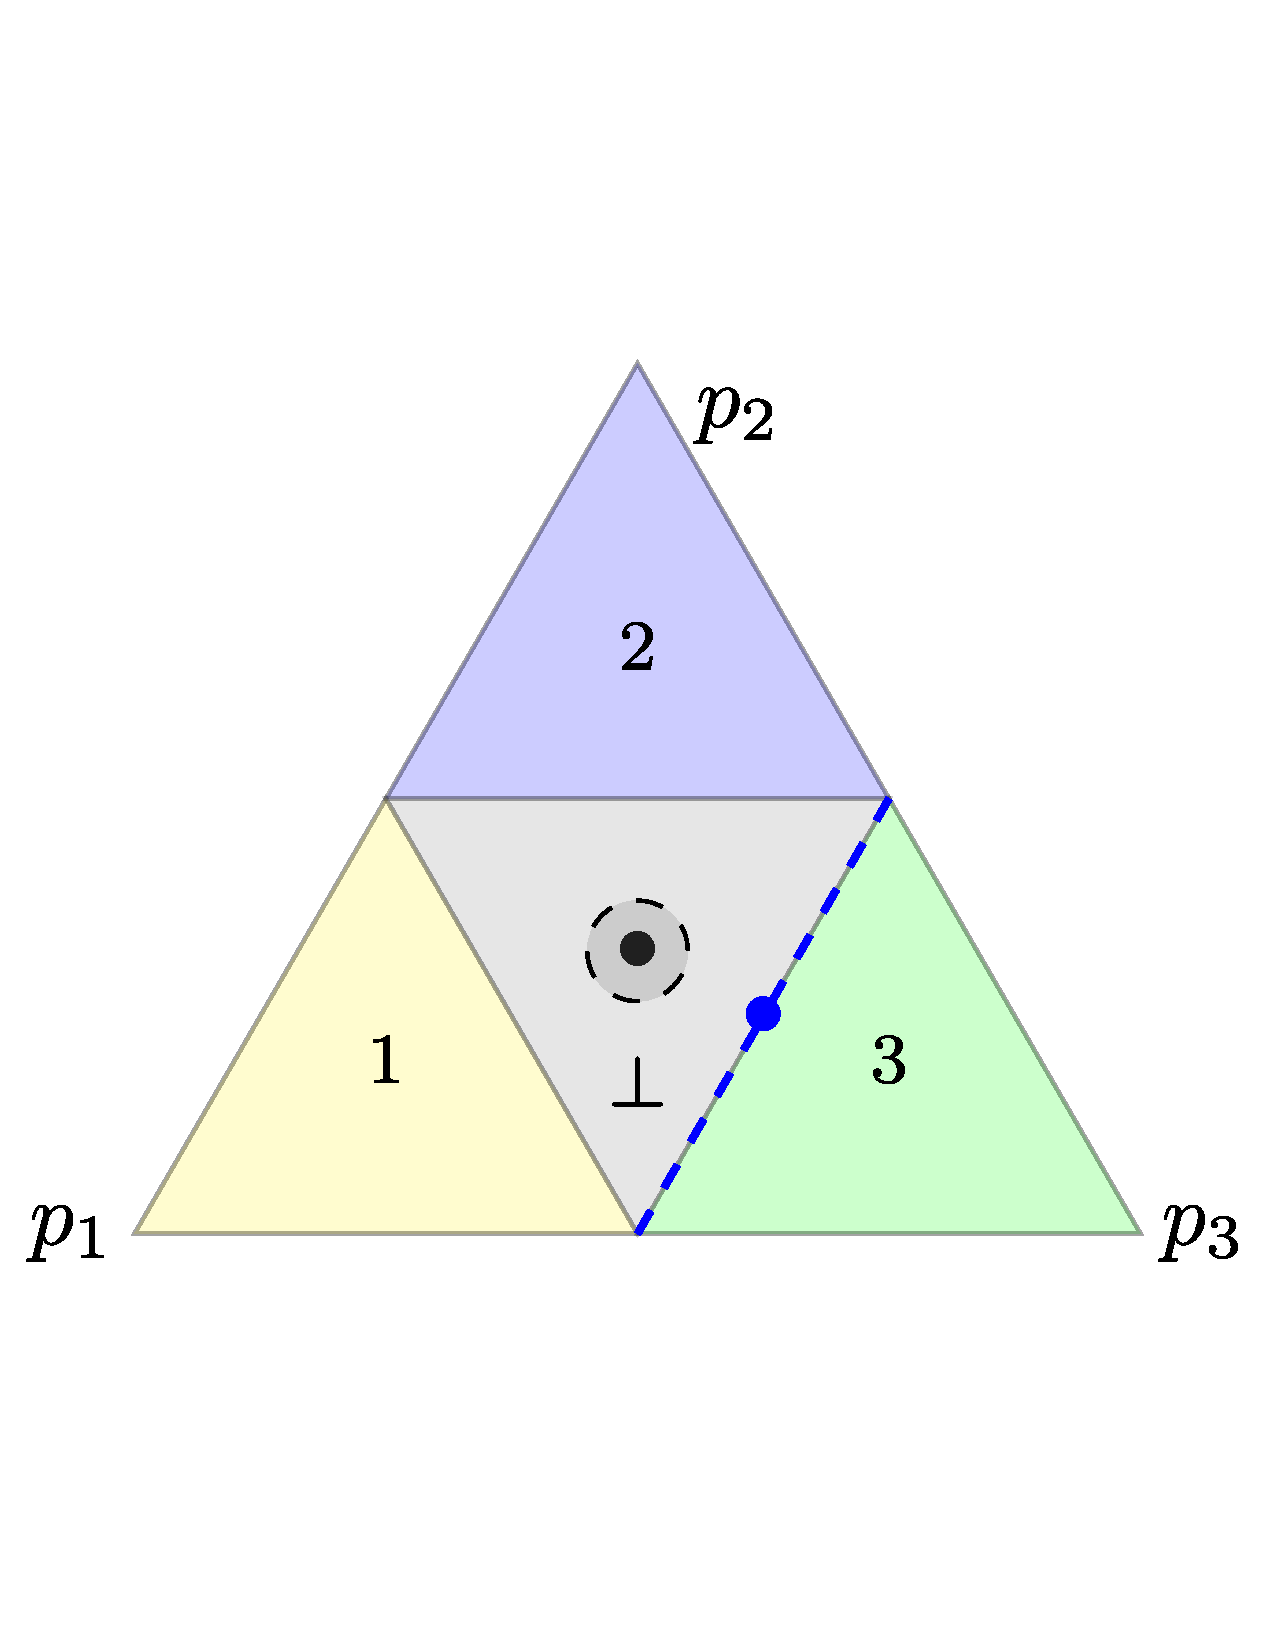
\includegraphics[width=\linewidth]{tikz/fsd-bound.pdf}
	\caption{Since the uniform distribution is on the relative interior of the simplex and the level set $\gamma_\bot$, its feasible subspace dimension is $2$. The distribution $p = (1/4, 1/4, 1/2)$ in blue has feasible subspace dimension $1$.}
	\label{fig:fsd-bound}
\end{minipage}
\hfill
\begin{minipage}{0.45\linewidth}
	\centering
	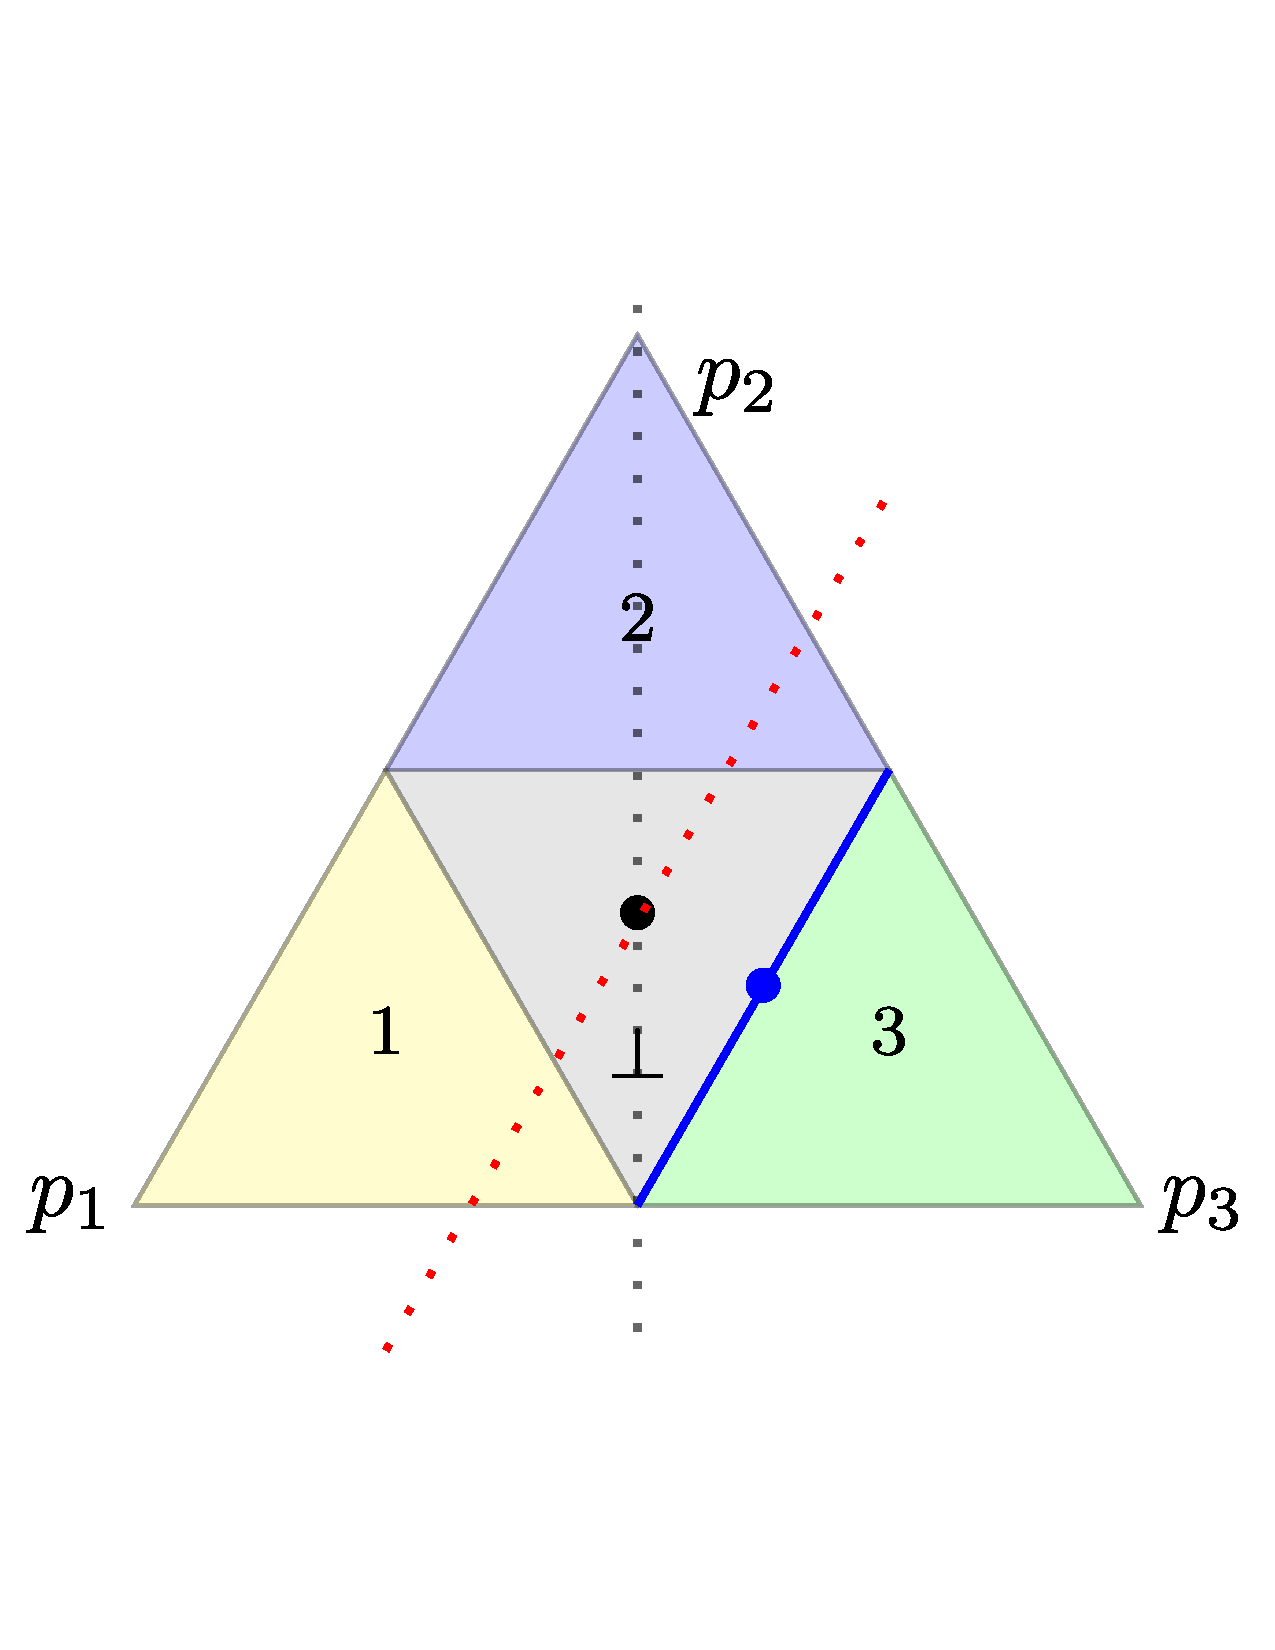
\includegraphics[width=\linewidth]{tikz/flats-bound.pdf}
	\caption{Any flat of codimension $1$ through the uniform distribution also leaves the (gray) cell $\gamma_\bot$ in the simplex. However, for the distribution $p = (1/4, 1/4, 1/2)$ in blue,there is a $1$ dimensional flat containing $p$ that is a subseteq of $\gamma_\bot$ and $\gamma_3$.}
	\label{fig:flats-bound}
\end{minipage}
\end{figure}

\section{Continuous-valued predictions}\label{sec:contin-consis}


Theorem~\ref{thm:consistent-implies-indir-elic} allows us to use convex elicitation complexity as a tool to understand efficiency of consistent convex surrogates for a given property, which is more often what is given in a continuous estimation setting.
For example, when one wants to learn an $\alpha$-quantile, we start with the property rather than a loss.
In the literature, pinball loss $L(r,y) = (r-y)(\ones_{r \geq y} - \alpha)$ typically appears without explanation or justification as to why it is relevant in relation to the $\alpha$-quantile.
Elicitation teaches us why pinball loss is consistent for learning a quantile as the pinball loss elicits the $\alpha$-quantile.


Theorem~\ref{thm:cvx-flats} also addresses one major open question from~\cite{frongillo2015elicitation,frongillo2018elicitation}\jessiet{which citation?}: \emph{what are lower bounds on convex elicitation complexity?}
While Theorem~\ref{thm:cvx-flats} is a statement about consistent surrogates, the heart of it is actually about indirect property elicitation.
Thus, the result also applies to extend previous results from~\cite{frongillo2015elicitation,frongillo2018elicitation} to provide new bounds on elicitation complexity for certain classes of properties in Theorem~\ref{thm:bayes-risk-lower-bound}.

\newcommand{\lbar}{\underline{L}} % couldn't do L* while proofreading...
\newcommand{\iden}{\mathrm{iden}}
\newcommand{\Var}{\mathrm{Var}}

\begin{lemma}[\cite{frongillo2018elicitation}]
  \label{lem:elic-complex-bayes-concave}
  Suppose the loss $L$ elicits $\Gamma:\simplex\to\R$.
  Let $\lbar$ be the Bayes risk of $L$.
  Then for any $p,p'\in\simplex$ with $\Gamma(p)\neq\Gamma(p')$, we have $\lbar(\lambda p + (1-\lambda) p') > \lambda \lbar(p) + (1-\lambda) \lbar(p')$ for all $\lambda\in(0,1)$.
\end{lemma}

% \begin{lemma}\label{lem:affhull-interior}
%   \raf{Skip this...}
%   Let $C\subseteq\reals^m$ be convex with nonempty interior $\mathring C$.
%   Then for any flat $F\subseteq\reals^m$ with $F\cap\mathring C \neq \emptyset$, we have $\affhull(F\cap C) = F$.
% \end{lemma}
% \begin{proof}
%   As $\affhull(F) = F$ and $F\cap C\subseteq F$, the inclusion $\affhull(F\cap C) \subseteq F$ is clear.
%   For the reverse, let $p\in F\cap\mathring C$ and let $B\subseteq C$ be an open set containing $p$.
%   For any $q\in F$, we thus have $q' = p + \epsilon (q-p) \in B$ for sufficiently small $\epsilon > 0$.
%   As $q' = (1-\epsilon) p + \epsilon q$, we have $q' \in \affhull(F)\cap C = F\cap C$.
%   As $q = (1-1/\epsilon) p + (1/\epsilon) q'$, we thus have $q\in\affhull(F\cap C)$.
% \end{proof}

\begin{lemma}\label{lem:affhull-relint}
  Let $C\subseteq\reals^m$ be convex.
  Then for any affine subspace $F\subseteq\affhull(C)$ with $F\cap\relint C \neq \emptyset$, we have $\affhull(F\cap C) = F$.
\end{lemma}
\begin{proof}
  As $\affhull(F) = F$ and $F\cap C\subseteq F$, the inclusion $\affhull(F\cap C) \subseteq F$ is clear.
  For the reverse, let $p\in F\cap\relint C$ and let $B\subseteq C$ be a relatively open set containing $p$.
  For any $q\in F \subseteq \affhull(C)$, we thus have $q' = p + \epsilon (q-p) \in B$ for sufficiently small $\epsilon > 0$.
  As $q' = (1-\epsilon) p + \epsilon q$, we have $q' \in \affhull(F)\cap C = F\cap C$.
  As $q = (1-1/\epsilon) p + (1/\epsilon) q'$, we thus have $q\in\affhull(F\cap C)$.
\end{proof}


% When extending the results of~\cite{frongillo2018elicitation}, we assume a property is identifiable, meaning its level sets are flats.
% \begin{definition}
%   A property $\Gamma:\simplex\to\R$ is \emph{$d$-identifiable} if its level sets are flats of co-dimension at most $d$ intersected with $\simplex$.
%   We write $\iden(\Gamma) = \min\{d \in \mathbb{N} : \Gamma\text{ is $d$-identifiable}\}$.
% \end{definition}

In the proof of Theorem~\ref{thm:consistent-implies-indir-elic} below, we modify the argument of~\citet[Corollary 7]{frongillo2018elicitation} to bound the elicitation complexity of the Bayes risk of the loss.
\raft{Note to self: need to sync the refs to the actual version on arxiv... or something...}
\begin{theorem}
  \label{thm:bayes-risk-lower-bound}
  Let $L$ elicit some $\Gamma:\simplex\to\reals^d$.
  Let $p\in\relint\simplex$ and let $\Gamma_r$ be some level set of $\Gamma$ such that
  (i) $p\in\Gamma_r$,
  (ii) $\codim(\affhull(\Gamma_r))=d$, and
  (iii) either $\Gamma_r$ is a singleton or $\lbar$ is nonconstant on $\Gamma_r$.
  Then $\eliccvx(\lbar) \geq \min(d+1,n-1)$.
\end{theorem}
\begin{proof}
  Suppose that we have some convex loss $\hat L:\reals^k\times\Y\to\reals$ eliciting a property $\hat\Gamma:\simplex\to\reals^k$, and link $\psi : \reals^k \to \reals$ such that $\lbar = \psi \circ \hat\Gamma$.
  % The condition $\iden(\Gamma)=d$ implies the existence of some level set $\Gamma_r$ such that $\codim(\affhull(\Gamma_r)) \geq d$; otherwise, taking $F_r = \affhull(\Gamma_r)$ for all reports $r\in\reals^d$, we would have $\codim(F_r) \leq d-1$ and $\Gamma_r = F_r \cap \simplex$, implying $\iden(\Gamma)\leq d-1$.
  The proof of \citet[Theorem 4]{frongillo2018elicitation} argues that $\hat\Gamma$ must refine $\Gamma$, in the sense that every level set of $\hat\Gamma$ is contained in a level set of $\Gamma$; for completeness we give the argument here.
  Suppose for a contradiction that we have $p,p'$ with $\hat\Gamma(p)=\hat\Gamma(p')$ but $\Gamma(p) \neq \Gamma(p')$.
  As $\lbar = \psi \circ \hat\Gamma$, we also have $\lbar(p) = \lbar(p')$.
  Letting $p'' = \tfrac 1 2 p +  \tfrac 1 2 p'$, Lemma~\ref{lem:elic-complex-bayes-concave} would then give us $\lbar(p'') >  \tfrac 1 2 \lbar(p) +  \tfrac 1 2 \lbar(p') = \lbar(p)$.
  By \citet{osband1985providing}, the level sets $\hat\Gamma_{\hat r}$ are convex, giving $\hat\Gamma(p'') = \hat\Gamma(p)$, which would imply $\lbar(p'')=\lbar(p)$, contradicting $\lbar = \psi \circ \hat\Gamma$.
  We conclude $\hat\Gamma$ must refine $\Gamma$, and thus $\hat L$ actually indirectly elicits $\Gamma$ through some other link function.
  % The proof of \cite[Theorem 4]{frongillo2018elicitation} argues that $\hat\Gamma$ must refine $\Gamma$, in the sense that for all $\hat r \in \hat\Gamma(\simplex)$ we have $\hat\Gamma_{\hat r} \subseteq \Gamma_r$ for some $r\in\reals^k$.

  By Theorem~\ref{thm:cvx-flats}, as $\hat L$ elicits $\hat\Gamma$ and indirectly elicits $\Gamma$, there is a level set $\hat\Gamma_{\hat r}$ and flat $\hat F\subseteq\affhull(\simplex)$ containing $p$ such that $\codim(\hat F) \leq k$ and $S := \hat F \cap \simplex \subseteq \hat\Gamma_{\hat r} \subseteq \Gamma_r$.
  \raft{This last statement does follow from the proof of our main theorem, but it takes a second to realize that we show the chain of inclusions. \jessie{Tried to clarify in that proof}}
  Let $F = \affhull(\Gamma_r)$ and recall $\codim(F)=d$.
  % Let $F' = \hat F \cap \affhull(\simplex)$, and observe the following: $p\in F'\cap\relint\simplex$, $F' \subseteq \affhull(\simplex)$, $S=F'\cap\simplex\subseteq\Gamma_r$, and $\codim(F') \leq k+1$.
  % the next \hat Fs used to be F's
  As $p\in \hat F\cap\relint\simplex$, Lemma~\ref{lem:affhull-relint} gives $\affhull(S) = \affhull(\hat F\cap \simplex) = \hat F$.
  Now as $S \subseteq \Gamma_r$, we also have $\hat F = \affhull(S) \subseteq \affhull(\Gamma_r) = F$,
  implying $\codim(\hat F) \geq \codim(F)$.

  If $\Gamma_r = \{p\}$ is a singleton, then $F = \affhull(\Gamma_r) = \{p\}$, and in particular $n-1 = \codim(F) \leq \codim(\hat F)$, so we must have $k=d=n-1$.
  If $\Gamma_r$ is not a singleton, suppose for a contradiction that $k\leq d$.
  Then $\codim(F) = d \geq k \geq \codim(\hat F)$, so we must have $\codim(\hat F)=d=\codim(F)$; combining with $\hat F \subseteq F$ gives $\hat F = F$.
  We now have $S = \hat F \cap \simplex = F \cap \simplex = \Gamma_r$, and as $S \subseteq \hat\Gamma_{\hat r} \subseteq \Gamma_r$, we conclude $S = \hat\Gamma_{\hat r} = \Gamma_r$.
  By assumption, $\lbar$ is non-constant on $\Gamma_r$, so we have distributions $p,p' \in \Gamma_r = \hat\Gamma_{\hat r}$ with $\lbar(p)\neq\lbar(p')$, which contradicts $\lbar = \psi \circ \hat\Gamma$.
\end{proof}


\subsection{Examples}

As a warm-up, let us see how to show $\eliccvx(\Var)=2$ whenever $|\Y|\geq 3$, meaning the lowest dimension of a convex loss to estimate conditional variance is 2.
It is interesting to note that, to the best of our knowledge, even this simple bound is novel.
While intuitively obvious, the lower bound of 2 is not trivial.
In particular, the well-known fact that the variance is not elicitable does not yield this lower bound, as it does not rule out the variance being a link of a real-valued convex-elicitable property; cf.~\citet{frongillo2018elicitation}.

Let $\Y\subseteq\reals$ be a finite set with $n=|\Y|$.
Observe that the variance of $Y$ is the Bayes risk of squared loss $L(r,y) = (r-y)^2$; as $L$ elicits the mean $\Gamma(p) = \E_p Y$, we have $\Var_p[Y] = \E_p (\E_pY - Y)^2 = \min_{r\in\reals} \E_p L(r,Y)$.
To apply Theorem~\ref{thm:bayes-risk-lower-bound}, we take this $L$ and $\Gamma$ and $d=1$, and must choose an appropriate level set $\Gamma_r$; we choose $p = \tfrac 1 n \ones$ to be the uniform distribution and let $r=\E_pY$.

Let us verify the three conditions:
(i) $p\in\Gamma_r$ by construction.
(ii) Letting $v\in\reals^\Y$ with $v_y = y - r$, define $F = \ker W \cap \affhull(\simplex)$ for $W = [v]\in\reals^{1\times n}$.
Note that $\Gamma_r \subseteq F$, and \raf{$W$ does not contain the $\ones$ direction}, as the $y$ values are distinct by assumption.
As $p\in F$, Lemma~\ref{lem:affhull-relint} gives $\affhull(\Gamma_r) = F$ and thus $\codim(\affhull(\Gamma_r)) = \rank(W) = 1 = d$.
(iii)
For $n \leq 2 = d+1$, $\Gamma_r=\{p\}$ is a singleton and we are done; otherwise $n\geq 3$.
\raft{I think we should punt this next bit to the appendix; it's pretty straightforward once you see what's happening, but really detracts from the simplicity of this example}
If $\Var[Y]$ were constant in $\Gamma_r$, then we would have some $c\in\reals$ such that $c = \Var_{p'}[Y] = \E_{p'} [Y^2] - r^2$ for all $p'\in\Gamma_r$.
Letting $W' = [v;v']\in\reals^{2\times n}$ where $v'_y = y^2-r^2-c$, and $F' = \ker W' \cap \affhull(\simplex)$, this would imply $\Gamma_r = F'\cap\simplex$ as well.
Lemma~\ref{lem:affhull-relint} applies again to show $F' = \affhull(\Gamma_r) = F$.
Yet as the $y$ values are distinct, $\rank(W')=2$ (for any $\alpha\in\reals$ there are at most two solutions to $y-r = \alpha(y^2-r^2-c)$), contradicting $\codim(F) = 1$.
Thus $\Var[Y]$ cannot be constant on $\Gamma_r$.

Applying Theorem~\ref{thm:bayes-risk-lower-bound} gives $\eliccvx(\Var) \geq \min(2,n-1)$, as desired.
In fact, this bound is tight for all $n$.
For $n=1$ there is only one distribution and we have complexity $0$; for $n=2$ the mean itself, elicited by squared loss, determines the distribution; for $n\geq 3$ we may elicit the first two moments via the convex $L(r,y) = (r_1-y)^2 + (r_2-y^2)^2$, and recover the variance via $\psi(r) = r_2-r_1^2$.

For another application, let us see how Theorem~\ref{thm:bayes-risk-lower-bound} implies $\eliccvx(G) = n-1$ for any strictly concave function $G:\simplex\to\reals$ of the distribution, including most entropy functions.
In other words, there is no convex loss function allowing one to consistently estimate conditional entropy using fewer dimensions than required to estimate the conditional distribution itself.
This observation also extends to norms; given any $k>1$, $G(p) = \|p\|_k^k$ is strictly convex, and hence $\eliccvx(\|\cdot\|_k) = n-1$, as otherwise we could link to $G$ via $\psi(r) = r^k$.
These results illustrate the power of our technique.

To show the bound, recall that $G$ is the Bayes risk of a proper loss defined by $L(p,y) = G(p) + s_p \cdot (\delta_y - p)$, where $\delta_y(y') = \ones\{y=y'\}$ is the point distribution on $y$ and $-s_p \in \partial (-G)(p)$ is a subgradient of $-G$ at $p$~\citep{gneiting2007strictly,reid2009surrogate,frongillo2014general}.
Intuitively, since $L$ elicits the identity property $\Gamma(p)=p$, Theorem~\ref{thm:bayes-risk-lower-bound} should therefore give us a maximal lower bound ($n-1$), as the level sets of are $\Gamma$ have codimension $n-1$.
For technical reasons, however, we need to drop a dimension from the prediction space, e.g.\ via the bijection $\varphi(p) = (p_1,\ldots,p_{n-1})$, defining $L'(p',y) = L(\varphi^{-1}(p'),y)$ which elicits $\Gamma'(p) = \varphi(p)$ but still has Bayes risk $G$.
Now the conditions of Theorem~\ref{thm:bayes-risk-lower-bound} are easily checked, where again $p\in\relint\simplex$ is the uniform distribution and $r=\varphi(p)$: (i) is trivial, (ii) $\codim(\affhull(\Gamma_r')) = \codim(\{p\}) = n-1$, and (iii) $\Gamma_r'$ is a singleton.
As with the variance example, the lower bound is easily matched, e.g.\ by $L_2(p',y) = \|\varphi^{-1}(p')-\delta_y\|_2^2$, which is convex in $p'$, and the link $\psi(p') = G(\varphi^{-1}(p'))$.


\section{Conclusions and future work}\label{sec:conclusions}
In this work, we show that indirect property elicitation can be studied as a necessary condition for the existence of a consistent surrogate loss (Theorem~\ref{thm:consistent-implies-indir-elic}).
Furthermore, we introduce a new lower bound (Theorem~\ref{thm:cvx-flats}) on the dimension of a consistent convex loss that is generally applicable and extends previous results from both the discrete prediction and continuous estimation settings.
Bounding the prediction dimension on convex surrogate losses may yield significant improvements in the complexity of the optimization algorithm as a whole.

While this work tightens bounds on the dimension of consistent surrogate losses, it does not completely characterize the dimensionality of a convex surrogate for a given problem.
One might be able to further tighten these bounds by property elicitation by studying monotonicity and adjacency of level sets.
In discrete predictions, these bounds might also be tightened if the equivalence of convex calibration dimension and embedding dimension of~\cite{finocchiaro2020embedding} is shown; the current embedding dimension bounds are not tight either, but additional structure is imposed by considering the embedding framework.
Lastly, the practical reason why consistency is desired is to ensure the guarantee of empirical risk minimization (ERM) rates; however, the relationship between ERM rates and property elicitation has not been studied.


\newpage

\section*{Broader Impact}
This work is entirely theoretical, thus the opportunity for broader impacts is indirect, but still present.
Understanding the complexity and efficiency of consistent, convex surrogates for different target losses and properties we wish to learn can lead to understanding the tradeoffs that are often made in ad-hoc surrogates that are not consistent.
These ad-hoc surrogates are consistent with respect to \emph{some property}, although it may not be the one we wish to elicit, either directly or indirectly.
As a general prediction task arises, one might be able to use property elicitation to understand what question they are actually answering (in the best base, with sufficient data that matches the real-world data distribution) by minimizing their surrogate loss and how it differs from the question they are actually trying to answer.

\begin{ack}
Nishant, Adam
\end{ack}

\bibliographystyle{plainnat}
\bibliography{diss,extra}

\newpage
\appendix
\section{A general notion of calibration}\label{app:calibration}
For general settings, we introduce a new notion of calibration that is a special case of calibration as introduced by~\cite[Chapter 3]{steinwart2008support}.
We will show that in discrete prediction settings, it is equivalent to the more commonplace definition given in Definition~\ref{def:calibrated-finite}.
Therefore, we use this more general definition of calibration when proving statements about the relationship between consistency, calibration, and indirect elicitation.

\begin{definition}[Calibrated]\label{def:calibrated-general}
	A loss $L:\reals^d \times \Y \to \reals$ is \emph{calibrated} with respect to a loss $\ell : \R \times \Y \to \reals$ eliciting the property $\gamma$ if there is a link $\psi : \reals^d \to \R$ such that, for all distributions $p \in \simplex$, there exists a function $\zeta : \reals_+ \to \reals_+$ with $\zeta$ continuous at $0^+$ and $\zeta(0) = 0$ such that for all $u \in \reals^d$, we have
	\begin{equation}\label{eq:calibrated-general}
	\ell( \psi(u); p) - \risk{\ell}(p)  \leq \zeta \left(  L(u;p) - \risk{L}(p) \right)~.~
	\end{equation}
\end{definition}

Consider the following four conditions: Suppose we are given $\zeta:\reals_+ \to \reals_+$.
\begin{enumerate}
	\item [A] $\zeta$ satisfies $\zeta : 0 \mapsto 0$ and is continuous at $0$.
	\item [B] $\epsilon_m \to 0 \implies \zeta(\epsilon_m) \to 0$.
	\item [C] Given $\zeta:\reals \to \reals_+$, for all $u \in \reals^d$, $R_\ell(\psi(u); p) \leq \zeta(R_L(u;p))$.
	\item [D] For all $p \in \simplex$ and sequences $\{u_m\}$ so that $R_L(u_m; p) \to 0$, we have $R_\ell(\psi(u_m); p) \to 0$.
\end{enumerate}
The existence of a function $\zeta$ so that $(A \wedge C)$ defines calibration as in Definition~\ref{def:calibrated-general}, and we show $A \iff B$ in Lemma~\ref{lem:continuous-iff-limits}.  
Lemma~\ref{lem:calib-converging-regrets} shows calibration if and only if $D$, which yields a condition equivalent to calibration without dependence the function $\zeta$.

\begin{proposition}
	When $\R$ is finite, a loss and link $(L, \psi)$ are calibrated with respect to a target loss $\ell$ via Definition~\ref{def:calibrated-general} if and only if calibration via Definition~\ref{def:calibrated-finite}.
\end{proposition}
\begin{proof}
	\jessiet{Old proof commented out; simplified using Lemma~\ref{lem:calib-converging-regrets}}
$\implies$
	We prove the contrapositive; if $(L, \psi)$ is not calibrated with respect to $\ell$ by Definition~\ref{def:calibrated-finite}, then it is not calibrated via Definition~\ref{def:calibrated-general} either.
	If $(L, \psi)$ are not calibrated with respect to $\ell$ by Definition~\ref{def:calibrated-finite}, then there is a $p \in \simplex$ so that $\inf_{u : \psi(u) \not \in \gamma(p)} L(u;p) = \inf_u L(u; p)$.
	Thus there is a sequence $\{u_m\}$ so that $\lim_{m \to \infty} \psi(u_m) \not \in \gamma(p)$ and $L(u_m; p) \to \risk{L}(p)$.  
	Now we have $R_L(u_m; p \to 0$ but $R_\ell(\psi(u_m); p) \not \to 0$, so by Lemma~\ref{lem:calib-converging-regrets}, we contradict calibration by Definition~\ref{def:calibrated-general}.
%	
% Commented out 05.19.2020 for easier proof if Lemma 5 is true.
%	We prove the contrapositive; if $(L, \psi)$ is not calibrated with respect to $\ell$ by Definition~\ref{def:calibrated-finite}, then it is not calibrated via Definition~\ref{def:calibrated-general} either.
%	
%	Suppose there was a distribution $p \in \simplex$ so that $\inf_{u : \psi(u) \not \in \gamma(p)} L(u;p) = \inf_{u} L(u;p)$.
%	There must then be a sequence $\{u_m\} \to u$ so that $\lim_{m \to \infty} \psi(u_m) \not \in \gamma(p)$ and $L(u_m; p) \to \risk{L}(p)$.
%	
%	This consequently implies $R_L(u_m;p) \to 0$ as $L(u_m; p) \to \risk{L}(p)$, but as $\ell(\psi(u_m); p) \not \to \risk{\ell}(p)$ (if it did converge, then we would have $\psi(u_m) \to r \in \gamma(p)$), so $R_\ell(\psi(u_m); p) \not \to 0$.
%	Thus, by Lemma~\ref{lem:calib-converging-regrets}, we have no calibration via Definition~\ref{def:calibrated-general}.  

$\impliedby$
Suppose there was a function $\zeta$ satisfying the bound in Equation~\eqref{eq:calibrated-general} for a fixed distribution $p \in \simplex$.
Observe the bound in Equation~\eqref{eq:calibration} can be written as $R_L(u,p) > 0$ for all $p \in \simplex$ and $u$ so that $\psi(u)$ is bounded away from $\gamma(p)$. \jessie{details correct??}

By Equation~\eqref{eq:calibrated-general}, for any sequence $\{u_m\}$ so that $\psi(u_m) \not \to \gamma(p)$, we have must have $\zeta(R_\ell(\psi(u_m), p)) \not \to 0$ as we would otherwise contradict the bound in Equation~\eqref{eq:calibrated-general} since $R_\ell(\psi(u), p) \not \to 0$. 
Therefore $R_L(u_m, p) \not \to 0$; thus, the strict inequality holds.
\end{proof}

The following Lemma shows that conditions $A$ and $B$ are equivalent, so that we can using condition $B$ in lieu of condition $A$ in the proof of Lemma~\ref{lem:calib-converging-regrets}
\begin{lemma}\label{lem:continuous-iff-limits}
	A function $\zeta:\reals \to \reals$ is continuous at $0$ and $\zeta(0) = 0$ if and only if the sequence $\{u_m\} \to 0 \implies \zeta(u_m) \to 0$.
	\jessie{$A \iff B$}
\end{lemma}
\begin{proof}
	$\implies$ Suppose we have a sequence $\{u_m\} \to 0$.
	By continuity, we have $\lim_{u_m \to 0}\zeta(u_m) = \zeta(0) = 0$, so $\zeta(u_m) \to 0$.
	
	$\impliedby$ Suppose $\zeta(0) \neq 0$ but $\zeta$ was continuous at $0$.
	The constant sequence $\{u_m\} = 0$ then converges to $0$, but as $\zeta$ is continuous at $0$, we must have $\lim_{m \to \infty}\zeta(u_m) = \zeta(0) \neq 0$, so $\zeta(u_m) \not \to 0$.
	
	Now suppose $\zeta(0) = 0$ but $\zeta$ was not continuous at $0$.
	There must be a sequence $\{u_m\} \to 0$ so that $\lim_{m \to \infty}\zeta(u_m) \neq \zeta(0) = 0$, so $\zeta(u_m) \not \to 0$.
\end{proof}

Lemma~\ref{lem:calib-converging-regrets} now gives a condition equivalent to calibration without requiring one to already have a function $\zeta$ in mind.
\begin{lemma}\label{lem:calib-converging-regrets}
	A continuous surrogate and link $(L,\psi)$ are calibrated (via definition~\ref{def:calibrated-general}) with respect to $\ell$ if and only if, for all $p \in \simplex$ and sequences $\{u_m\}$ so that $R_L(u_m; p) \to 0$, we have $R_\ell(\psi(u_m); p) \to 0$.
	\jessie{$(A \wedge C) \iff D$}
\end{lemma}
\begin{proof}
\jessie{$(A \wedge C) \implies D$}
	$\implies$ Take a sequence $\{u_m\}$ so that $R_L(u_m;p) \to 0$.
	Since $\zeta(0) = 0$ and $\zeta$ is continuous at $0$, we have $\zeta(R_L(u_m;p)) \to 0$.
	As the bound from Equation~\eqref{eq:calibrated-general} is satisfied for all $u \in \reals^d$ by assumption, we observe
	\begin{align*}
	\forall m, \; &0 \leq R_\ell(\psi(u_m); p) \leq \zeta(R_L(u_m;p))\\
	\implies &0 \leq \lim_{m \to \infty} R_\ell(\psi(u_m); p) \leq \lim_{m \to \infty} \zeta(R_L(u_m;p)) = 0\\
	\implies &0 = \lim_{m\to\infty} R_\ell(\psi(u_m); p) ~.~
	\end{align*}
	
	
	$\impliedby$ 
\jessie{$D \implies (A \wedge C)$}
	Fix $p \in \simplex$, and consider $\zeta(c) := \sup_{u: R_L(u;p) \leq c} R_\ell(\psi(u); p)$.  
	We will show $R_L(u_m; p) \to 0 \implies R_\ell(\psi(u_m); p) \to 0$ gives calibration via the function $\zeta$ constructed above. 
	With $\zeta$ as constructed, we should that the bound in equation~\eqref{eq:calibrated-general} is satisfied for all $u \in \reals^d$ and apply Lemma~\ref{lem:continuous-iff-limits} to observe that if there is a sequence $\{\epsilon_m\} \to 0$ so that $\zeta(\epsilon_m) \not \to 0$, it is because $R_L(u_m, p) \not \to 0 \not \implies R_\ell(\psi(u_m), p) \to 0$.
	

\jessie{D $\implies$ C}
Now, we observe that the bound in Equation~\eqref{eq:calibrated-general} is satisfied for all $u \in \reals^d$ by construction of $\zeta$.
Let $S(v) := \{u' \in \reals^d : R_L(u';p) \leq R_L(v,p) \}$.
Showing $R_\ell(\psi(u);p) \leq \sup_{u' \in S(u)} R_\ell(\psi(u') ; p)$ for all $u \in \reals^d$ gives the condition $C$.
As $u$ is in the space over which the surpremum is being taken (as $R_L(u;p) \leq R_L(u;p)$), we then have calibration by definition of the supremum.

\jessie{Not $B$ leads to contradiction of $D$.}
Now suppose there exists a sequence $\{\epsilon_m\} \to 0$ so that $\zeta(\epsilon_m) \not \to 0$.
Consider $S(\epsilon) = \{u \in \reals^d : R_L(u,p) \leq \epsilon\}$.

\begin{align*}
\epsilon_1 \leq \epsilon_2 &\implies S(\epsilon_1) \subseteq S(\epsilon_2)\\
&\implies \zeta(\epsilon_1) \leq \zeta(\epsilon_2)~.~
\end{align*}
Now suppose there exists a sequence $\{u_m\}$ so that $R_L(u_m, p) \to 0$.
Then for all $\epsilon > 0$, there exists a $m' \in \mathbb{N}$ so that $R_L(u_m, p) < \epsilon$ for all $m \geq m'$.
Since this is true for all $\epsilon$, we have $S(\epsilon)$ nonempty for all $\epsilon > 0$, and therefore $\zeta(c)$ is discrete for all $c > 0$.
Now if $\zeta(\epsilon_m) \not \to 0$, it must be because $R_\ell(\psi(u_m), p) \not \to 0$ for some sequence converging to zero surrogate regret, and therefore we contradict the statement $R_L(u_m, p) \to 0 \implies R_\ell(\psi(u_m), p) \to 0$.

Moreover, we argue that such a sequence of $\{u_m\}$ with converging surrogate regret always exists by continuity and boundedness from below \jessiet{really just need lower semi-continuity and boundedness from below} of the surrogate loss, since we can take the constant sequence at the (attained) infimum.
%
%\jessie{$D \implies A$, but actually $\lnot B \wedge C \implies \lnot D$}
%Fix $p \in \simplex$.
%Suppose we have a sequence $\{\epsilon_m\}$ so that $\epsilon_m \to 0$, but $\zeta(\epsilon_m) \not \to 0$.
%If $L$ is continuous over the reals \jessiet{Need this, right?}, then for each $m$, we can construct a subsequence $\{u^j_m\}$ so that $R_L(u^j_m, p) \to \epsilon_m$ for all $m$.
%We can now construct the sequence $\{\epsilon'_m\}$ with $\epsilon'_m = \lim_{j \to \infty} R_L(u^j_m, p)$.
%This sequence converges to $0$, but we have $\lim_{m \to \infty} \zeta(\epsilon'_m) = \lim_{m \to \infty} \lim_{j \to \infty} \zeta(R_L(u^j_m, p)) \not \to 0$. 
%As $R_\ell(\psi(u_m); p) \leq R_L(u_m; p)$ for all $m$, we then have this being true in the limit.
%For this sequence, this then gives a loose bound of $0 \leq \lim_{m\to\infty} R_\ell(\psi(u_m); p) \leq c$. 
%	
\end{proof}

\subsection{Relating calibration, consistency, and indirect elicitation.}
Even with the more general notion of calibration that extends beyond discrete predictions, we still have consistency implying calibration.
\begin{proposition}\label{prop:consistent-implies-calibrated}
	If a loss and link $(L, \psi)$ are consistent with respect to a loss $\ell$, then they are calibrated with respect to $\ell$.
	\jessiet{Probably appendix later; also, should this be a lemma instead of a proposition?}
	%  \raft{Do we define ``continuous loss''?  Maybe ``(not necessarily discrete)'' is clearer.}
\end{proposition}
\begin{proof}
	We show the contrapositive.
	If $(L, \psi)$ are not calibrated with respect to $\ell$, then there is a sequence $\{u_m\}$ such that $R_L(u_m; p) \to 0$ but $R_\ell(\psi(u_m); p) \not \to 0$ via Lemma~\ref{lem:calib-converging-regrets}.
	Suppose $D \sim \X \times\Y$ has only one $x \in \X$ with $Pr_D(X = x) > 0$ so that $p := D_x$ and $\E_D f(X,Y) = \E_p f(x, Y)$.
	Consider any sequence of functions $\{f_m\} \to f$ with $f_m(x) = u_m$ for all $f_m$.
	\raft{Type error with $D=D_x$; see AA15 for how they phrase \jessie{better?}}
	Now we have $\E_D L(f_m(X), Y) \to \inf_f \E_D L(f(X), Y)$, but $\E_D \ell(\psi \circ f(X), Y) \not \to \inf_f \E_D \ell(\psi \circ f(X), Y)$, and therefore $(L, \psi)$ is not calibrated with respect to $\ell$.
\end{proof}

Moreover, we have calibration implying indirect elicitation.
\begin{lemma}\label{lem:calib-implies-indir}
	If a surrogate and link $(L, \psi)$ are calibrated with respect to a loss $\ell:\R \times\Y \to \reals$, then $L$ indirectly elicits the property $\gamma := \prop{\ell}$.
\end{lemma}
\begin{proof}
	Let $\Gamma$ be the unique property directly elicited by $L$, and fix $p \in \simplex$ with $u$ such that $p \in \Gamma_u$.
	As $p \in \Gamma_u$, then $\zeta(L(u;p) - \risk{L}(p)) = \zeta(0) = 0$, we observe the bound $\ell(\psi(u); p) \leq \risk{\ell}(p)$.
	We also have $\ell(\psi(u); p) \geq \risk{\ell}(p)$ by definition of $\risk{\ell}$, so we must have $\ell(\psi(u);p) = \risk{\ell}(p) = \ell(\gamma(p); p)$, and therefore, $p \in \gamma_{\psi(u)}$.
	Thus, we have $\Gamma_u \subseteq \gamma_{\psi(u)}$, so $L$ indirectly elicits $\gamma$.
\end{proof}

Combining the two results, we can observe the result of Theorem~\ref{thm:consistent-implies-indir-elic} another way: \emph{through calibration}.

\section{Omitted Proofs}\label{app:omitted-proofs}
\begin{proposition}\label{prop:elic-cplx-lb-ccdim}
	Consider the discrete loss $\ell : \R \times \Y \to \reals_+$ and $\gamma:= \prop{\ell}$.
	Then $\eliccvx(\gamma) \leq \ccdim(\ell)$.
\end{proposition}
\begin{proof}
	Let $d$ be the convex calibration dimension of $\ell$, and $(L, \psi)$ be calibrated with respect to $\ell$ with $L$ convex.
	Then $L$ indirectly elicits $\gamma$ by Lemma~\ref{lem:calib-implies-indir}.
\end{proof}


\end{document}

%%% Local Variables:
%%% mode: latex
%%% TeX-master: t
%%% End:
